\documentclass[onecolumn]{book}

\title{The Hollow Mountain III}

\author{Tanguy Racine}
\usepackage{graphicx}
\usepackage{grffile}
\usepackage{caption}
\usepackage{subcaption}
\usepackage{cite}

\begin{document}
\maketitle

\chapter{2013- Z Mig na Kuk} 
\begin{flushright}
\huge \it From Mig to Kuk
\end{flushright}

\section{Slinging in the Rain}
 \begin{verse}
Rhys Tyers
\end{verse}

\chapter{2014 - Zkosi Zrcalo} 
\begin{flushright}
\huge \it Through the looking glass
\end{flushright}

\section{Preparing the ground for another camp}
\begin{verse}
Jarvist Frost
\end{verse}
\subsubsection{August 5, 2014 --- Prelude}
With a new job in Bath, yet still one half of my life in London, I hurtled towards the summer with some severe time restrictions and I feared that I would not be able to make it to the expedition. After some time staring into my soul, I withdrew an abstract from a conference and booked some cheap flights Bristol toTreviso. All I could line up was ten days, 25th July to the 4th August.

I made it to London the weekend before the van left, and joined in with the last minute preparations ? pushing trolleys around Clapham Lidl and ASDA, filling our boots with cut price carbohydrates and ready munch. We then had a full day in stores, helping deal with the too-long and yet ill-defined and nebulous ToDo list. A big oversight was that the underground camp gear had remained unwashed since the previous summer, and so required many hours of laundry room attendance as the sleeping bags and comf were washed and then extensively tumble dried before being packed for -550 m.

My drone (a Hubsan H107C HD Camera quadcopter) arrived in time to be sealed in a mini Daren drum with my XML bike light, but not much tested. It fits wonderfully in a small Daren drum with a few roll-mat circles of padding. The controller actually clips within the bottom ring, and the rotor cage of the quadcopter similar sits gently against the narrowing for the neck.
Arrival

The flight out was pleasant, but I had a lot of travelling to do in Europe. From Treviso I walked to the train station to catch one of the every two-hour trains towards Gorizia. Jackie's pub, just near the airport, served good pizza on the way back. From Treviso I trained to Gorizia, caught the 1-Euro international bus across the border to Nova Gorica (bus station), and then caught the evening bus to Tolmin. I arrived in time to meet Tetley, Martin, Janet and friend, and go out for Pizza.

The next morning, Janet had very kindly offered to get up early (6:30!) and drive us to Ravne in her hire car. This was a great boon, and two carries later I was firmly ensconced upon the mountaintop. Unfortunately, my timings did not mesh with the expedition. Many people were leaving that weekend, and so most cavers headed down to Tolmin. I spent my time on Sunday doing a food carry, and generally fettling. The weather during my time there was appalling ? almost no sun, clag or heavy rain the rest of the time. At least it was fairly warm!
Action

Rhys had returned, and we had a plan to go caving (a 3 day camp) on Tuesday, which would form the totality of my expedition. The weather was horrific, rain and clag which made it difficult to muster the enthusiasm to go caving, or to prepare gear and pack Daren drums. We decided to rotate onto the Night Train (i.e. sleep during the day) due to our slipping timings, and to make more considerate use of the 4-bed camp at X-Ray. We had a hare-brained plan to setup a full blown mini camp at Red Cow, but the amount we would have to take down (and take out) was prohibitive; and there were no more club 4-season sleeping bags so would be very cold. There was also the obvious safety implications of camping away from the others, with potentially no contact for days (i.e. no daily callout). Dan Greenwald had done a bounce trip to X-Ray on Monday, replenishing the camp with supplies and removing rubbish.

Our plan was to spend all the time near Red Cow, emplace a tent and roll mats for a camp, get down to Watership down and push the dry leads near the sump, and sort out as much of the rigging between X-Ray and the sump to support a possible diving expedition next year.
After supper and a break in the weather, we set off for the cave entrance in the gathering dusk. We had two tackle sacks each.

Jarv:
\begin{itemize}
\item Daren with photo equip, survey gear, sonar + laser rangefinder, chocolate bars, music speakers. Mini Daren with drone + bike light. Additional Uneo drill and two batteries, spare 8mm bits.
\item 2 man single-skin tent, wrapped up in a roll mat
\end{itemize}

Rhys:
\begin{itemize}
\item Daren for camp with food, candles, spare batteries etc.
\item Roll mat, with a core of food packed in plastic bags and fuel for the stove.
\end{itemize}


\subsubsection{Day 1}
Smooth trip down to camp, where we repacked and ate some hot food (William and Tanguy were on the day-train at a similar time, coming down to sleep then push tomorrow).
We set off with tent, roll mats and drill (with single battery), intending to stay above Republica and sort the rigging.
The night train dragged, as it always does. The drill would not work, though we couldn't tell whether it was the (single) battery or the drill itself. Disappointing. We rebolted the freeclimb at the end of memory lane with Spitz.
We then progressed to Red Cow, found a good space for the tent (slightly further along the passage, in 'Nevermore'). This is a wonderful camping spot. The passage is broad and dry (as in, oversuits seem to dry quickly there), with fine rock-flour 'sand', a solid phreatic ceiling and smooth exposed rock with useful shelves. It's particularly picturesque, with what appear to be large limpet-like fossils in the ceiling, and then a series of solution Oxbows further along.

The new 2-man tent at Red Cow
We located a latrine for camp, another ~30m along the passage. Here a small phreatic leads down a too-small to push lead for about 5m. You could even use it as a long drop toilet, depending what you were planning to do with excrement? However, the first thing to go down it was one of my gloves (brand new, and super warm Marigold Astroflexes). I had placed them within my oversuit while cooking (to keep them warm), but forgotten about them, and then approached the latrine with sufficient momentum (and lack of care) that when I ripped open the velcro of my oversuit, one was catapulted into the breach, and I watched helplessly as it did a Jacob's ladder tumble to the ~5m depths of the hole.

It was now approaching 4 AM and time was seriously beginning to drag. X-Ray camp times were 8-8 this year, coming back early is extremely disruptive to the previous shift's sleep. After our coffee and lunch, we crawled into the tent (wearing full kit, minus harness and helmet) and had a little rest. Nicknamed 'Camp Cuddle' (for this year only), Rhys reckons he didn't get any sleep, but I distinctly remember him snoring.

I find it really interesting that a tent (to shield from the draft, and retain warm air) and roll mats (to insulate from the cold rock) were sufficient to make the conditions survivable (if not pleasant). Certainly we would not have been falling asleep had we been cowering in survival bags.
Anyhow, the next time I looked at my watch it was 6:30 AM and we were pretty chilled. We quickly put our gear back on, and set off at speed back towards camp. We covered the ground in 90? (one bag each), moving quickly at the start as we were desperately trying to warm up!
Back at X-Ray we were pretty exhausted. Tanguy very kindly made us tea + some supper, though neither of us were hungry ---the night train really messes up both your hunger and sleep cycles.

\subsubsection{Day 2}
We packed for the depths, and figured out that it was the drill we had brought down (with dodgy wiring) rather than the batteries. William kindly carried out the dodgy drill and we packed for the bottom of the cave, with as many odd lengths of rope and sufficient hangers / bolts that we could muster. Everything was a bit minimal at X-Ray, with fewer finds this year we hadn't seen the bulk supply of rope and equipment that occurred in previous ones. Metalwork had to be separated from bags where it was stored with carbide to keep it dry over the winter.
We went direct to Republica, leaving the drill and food at Red Cow, and were suitably awed by the water levels. The chamber was very spray lashed, and a lot of water was going down the pitch ? the waterfall going directly via where the rope hung!
So we started hand bolting to the right, avoiding the water. I put the two traverse bolts in while sucking teeth and muttering about the quality of the ceiling rock. Rhys, in his PVC, went over the edge, fixed a temporary deviation (we had no skyhook), and thereby slithered around further to the right into a cubby hole on the pitch and rigged down a dryish route, on our new 10mm gold rope. We munched a chocolate bar, and headed back to Red Cow taking photos in Republica and the streamway (I was very cold, Rhys was splashed after having stomped around the bottom of Republica). This was rather difficult due to the sheer amount of spray flying about!

At Red Cow we had a hot drink and some food. I decided the conditions really were too wet to have much of a chance of reaching the sump ? Insomnia was likely to be wetter than Republica, and a lot of Day Dreamers puts you very close to the stream.

So we decided to curtail our attempt on Watership Down for the day, and instead rig our way back to X-Ray with the now fixed drill and battery combination. This was after another snooze at Camp Cuddle, where Rhys woke rather angrily after 90? of sleep (when I woke and looked at my watch), believing that he'd only been in the tent five minutes!
We collected all the ~2010-2011 ropes left at Red Cow, and returned to X-Ray photographing and rerigging. We placed our full complement of 8 rawl bolts, forming Y-hangs where they'd been dodgy natural over-hangs, traverse lines where there were trip wires and SRT options where previously only brute force would do; and of course photographing as we went.


\begin{figure}[h]
\centering
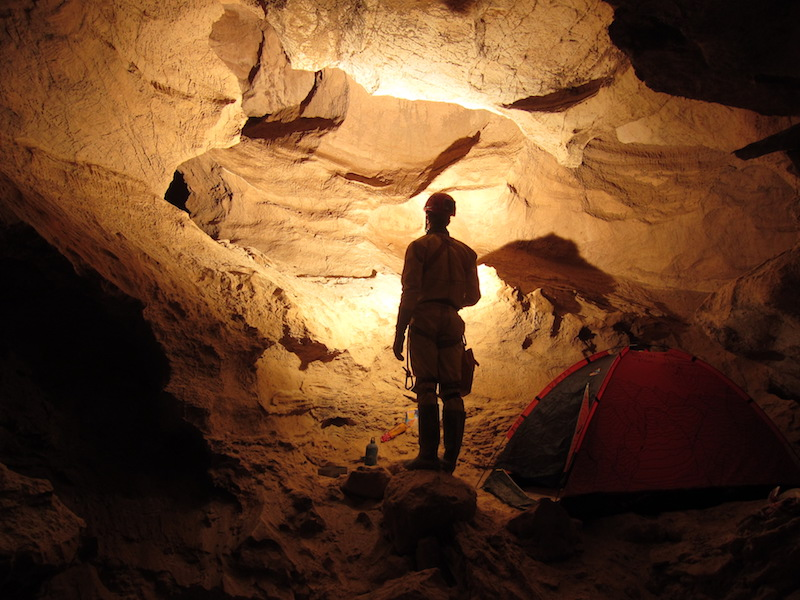
\includegraphics[width=\textwidth]{Rhys Red Cow.jpg}
\caption{Rhys Tyers at Red Cow camp --- Jarvist Frost}
\label{rhys red cow}
\end{figure}


\subsubsection{Day 3}
During the night, Andrej and Dan arrived to visit Roaring, but came back early at 5 and had supper then a snooze in the spare sleeping pits. When we got out of bed at 8, Zimmer was still roaring ('like a Hydro Turbine' ? Andrej) and so we put to bed our plans to visit Watership Down. Instead we packed laser disto, camera gear, the drone, and a proper lunch, and aimed the controls for Strap on the Nitro (Aven) and beyond.

A speedy trip to Red Cow admiring our new string, where we dumped the food and the stereo, pared our collection down to a single bag and continued to Strap On.
From Red Cow it was up a rift to an enormous stacked boulder (I wonder if anyone dared climb past it to see if there's a continuation?) then back down to more powder-filled passage, a small pitch, an abandoned 2004 tacklesack that appeared stuffed with rope and rigging (more on this later?), and a scary freeclimb down a beautiful cliff face to reach the note demarking Strap On.

The aven is impressive: 33m with the laser disto, smooth good quality rock at 70 degrees to the horizontal, Tetley's + Tom's escape route rigged off a nodule at about +12m, and a good draft disappearing up the aven.
We unpacked the flash and took a few photos, then got the drone out. Rhys was the WW2 'searchlight' operator with my 2xXM-L lithium ion bike light. I flew the drone.
The experience was rather exciting; control was on a knife edge. I had intended to have a few different micro-SD cards, and to swap them between flights so that if I got the beast stuck up the aven, I'd still have all but the latest footage. Alas, I wasn't organised enough, so I was extremely wary of losing it.

The first flight I had a look around at up to about 20 m off the floor, checking that the controls were working. The second flight I took it straight up to near the top of the aven. Here it seemed like I was having to fight against a wind that was attempting to take me into and over to the left of the aven. Drops hitting the craft were extremely destabilising to the control system, making it pitch and precess around until recovering. After these two flights I decided we'd probably had our luck.

We then continued into potato ? a lovely bit of cave with large tunnels and white powder floors, nice pitches (OK; natural belays and old 9mm again, scary). I glanced at my watch and noticed that it was passing midnight on July 31st ? so informed Rhys that his two year reign as president was over (?The King is dead, long live the King!?).
The low point you pass through (~potato.23) is particular interesting, as it's got obvious features of being a river bed, with a bank of water-abraded pebbles which you crawl over.
From potato.18 you make a long and consistent assent to the end, passing over one up-pitch. The passage seems fault controlled, with sections of perfectly level bedrock.


This is the end of the 2003 pushing, and the start of Smash. This was really quite nasty ? you start with a severe climb into an area of breakdown and boulder choke, no more white powder just angular rocks and mud. There are a few carbide arrows, but not enough to make you confident. I'm fairly certain things have moved since 2004. The area is very unstable. In the final chamber, we found the squeeze onto a pitch (blackness) which Dan had warned us about, but managed to find an earlier way through the boulders which reached a freeclimb down a steep boulder slope, to a PSS note 'did you like the squeeze?'. We could see the Spitz on the wall for the squeeze then pitch, but there was no rope. This was very odd, and quite discombobulating.

Miles Underground was OK, being mainly wide rift passage with boulder hopping. There were a few places where you could look back + up in the rift, many possible leads. Again it wasn't super stable. It ended at a short pitch down, again derigged! The PSS talked about an undescended pitch down by a waterfall, which we could certainly hear.
Rhys found a bypass by doubling back on the right and climbing through the boulders ? tight but passable, and completely without wear.

We were now in Beyond. After a fairly large boulder slope with the waterfall in the corner, this returned to a large-rift development, except for an obvious bit which appeared to be a fault-controlled bit of phreatic, with crack in the floor and then symmetric tulip profile either side. In ~3m wide rift we came across the Rock of Sages ? not as big as depicted on the survey!
After more rift we reached the obvious end of Beyond. The passage just continues in rift that turns into a climb on massive blocked boulders ('To Infinity and Beyond') though I'm not sure I would call it an aven!

The obvious way on here was a steep, again geomorphically controlled, slope of pure white limestone at about 60 deg to the horizontal and perhaps 10-15 m width. The roof was ~2m away, and seemed a different, darker and more structured limestone. It was an easy descent, but I had qualms about the return.
This shallowed out into a beautiful 5 m across phreatic. After some descent, an immature stream entered on the right and started running along a ~5 cm wide crack in the solid rock floor. The passage continued to a 90 degree bend to the left, where a similar sized passage issued a similarly sized stream from directly ahead. I believe this is around colarado.10 on the survey, but there were no PSS down here. I don't believe this passage has been pushed.

The combined streams continued down, and our phreatic merged with an almost identical one running in fromt the right, us having to step sideways between areas of boulders and confusion. (I believe this forms the 'Hoover Dam', but we did not follow it).
The last run to the 'sump' is absolutely dead straight (for greater than the 40 m limit of the laser disto), with about a 1 in 3 slope, and with the now ~10 cm wide stream running in its own slot back and forwards across the floor. It had taken us 3.5 hours to reach Colarado starting in X-Ray, including playing in Strap On. Yet it felt a lot further.
The passage then flattens out, the water entering a pool mostly choked with fine rock flour which has formed a perfectly levelled silt bank which is dense enough to walk on. The PSS was on a little cairn, about 20 cm above the water level. It's pages were covered with silt deposits, but it wasn't massively disturbed ? suggesting the water does occasionally backup, but never flows aggressively.

The plan shape of the passage is a hammer head, there are alcoves on the left and right with the thin crack of a fault line. The silt bank lead through a rock arch to within the 'sump', so I stooped and ducked in.

\begin{figure}[h!]
\centering
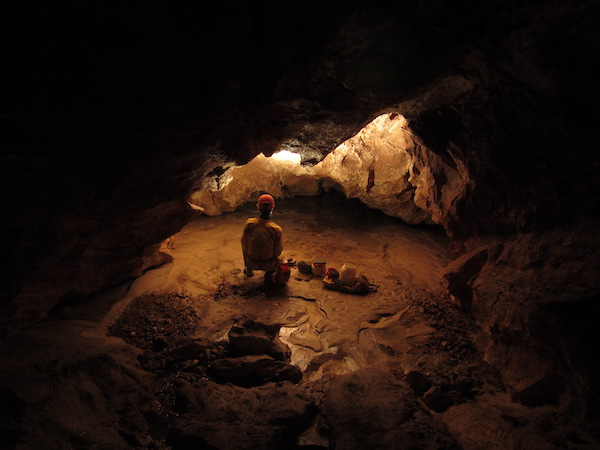
\includegraphics[width=\textwidth]{Rhys Colarado Sump.jpg}
\caption{The Colarado 'duck' from higher in the passage --- Jarvist Frost}
\label{Colarado Duck}
\end{figure}

\begin{figure}[h]
\centering
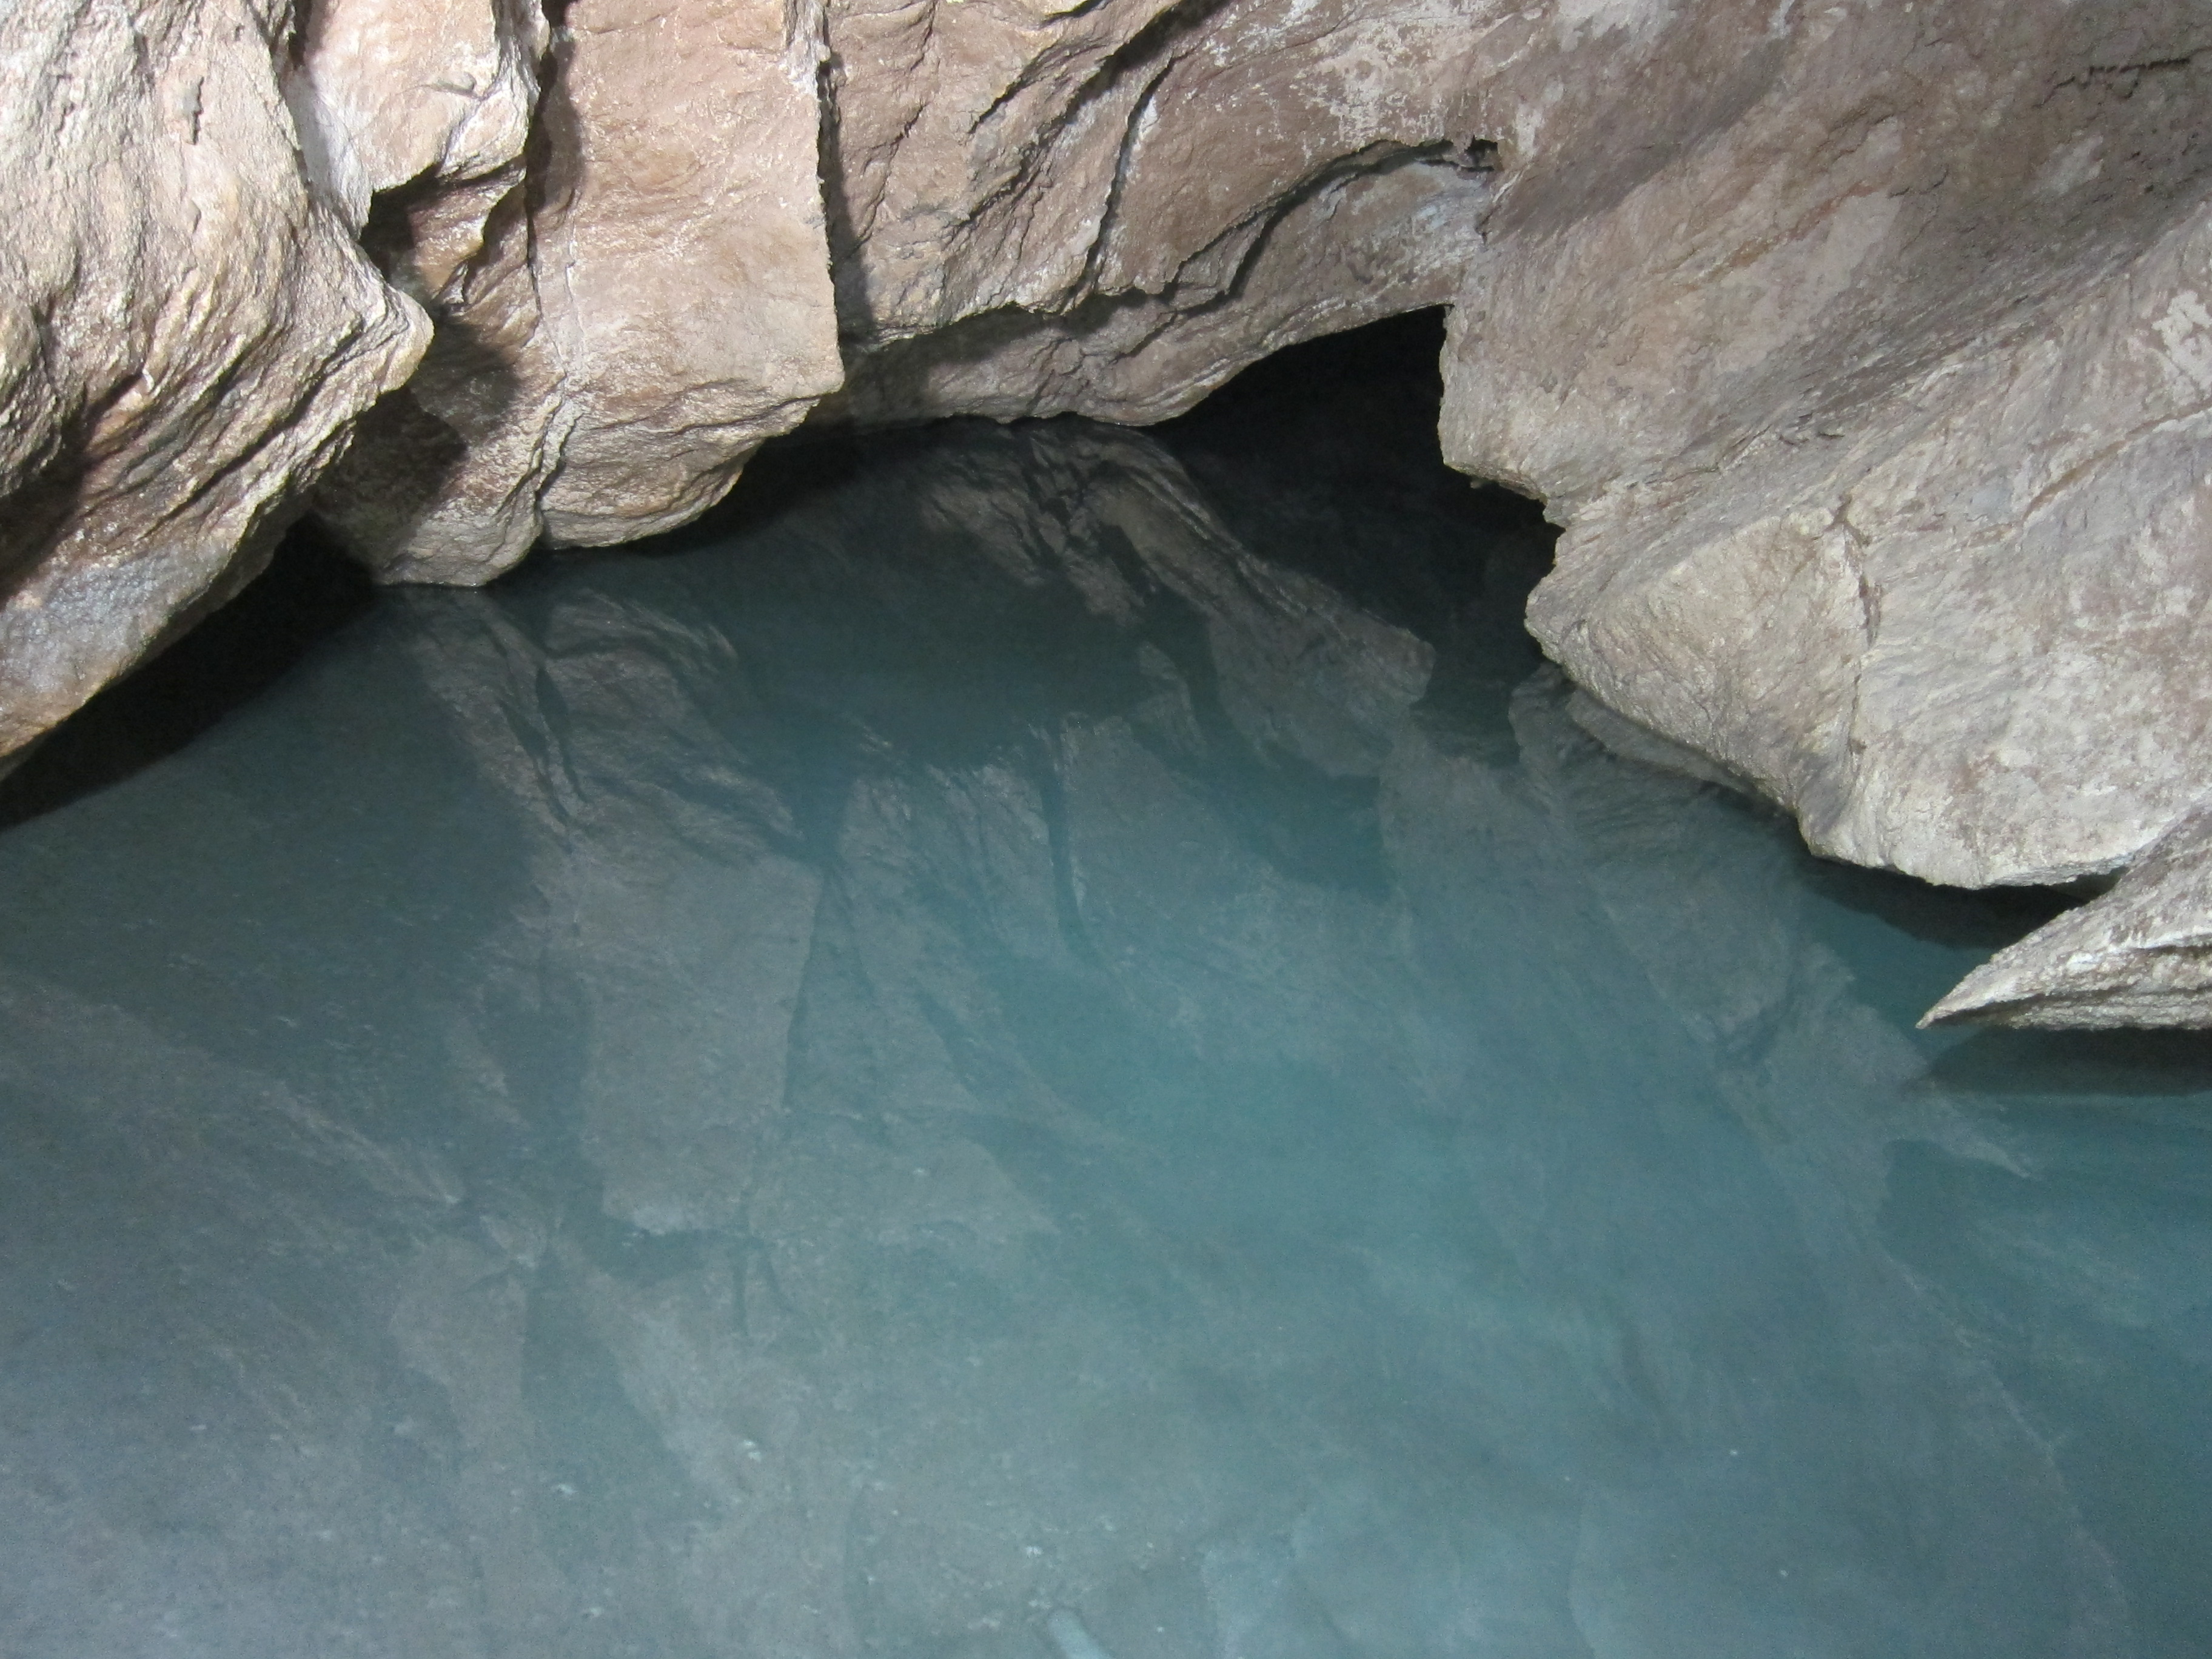
\includegraphics[width=\textwidth]{Colarado Duck.jpg}
\caption{The Duck proper --- Jarvist Frost}
\label{Duck from close up}
\end{figure}

\begin{figure}[h!]
\centering
\includegraphics[width=18cm, angle=270]{Hourglass passage.jpg}
\caption{Rhys Tyers in a \lq Hourglass Passage' near Leprechaun --- Jarvist Frost}
\label{Hourglass Passage}
\end{figure}

The first thing I noticed was the echo ? it sounded like a much larger chamber. Looking along the azure surface, there was an obvious black rock arch, seemingly about 4 m away, 40 cm across and 30 cm high above the water surface. The profile of the sump seemed to be roughly bath-tub.
I went and got camera and laser disto. By nearly touching my face to the water I could look through the arch, and see to the far side. There was a boulder at the water's edge, and slope leading up behind it. Slightly to the right of the boulder was what looked like a beach of silt or pebbles. The laser disto measured 14 m through to the other side, with 3 m from the PSS to where I was standing within the 'sump'. The air was totally still, so the passage must be sumped.

From the extremely well defined 5m across phreatic, my belief is that this duck is perched, and that the phreatic has been disrupted by a slip-fault running across it. I would not be surprised if the person to first pass this duck will find a continuation of the phreatic leading down towards the water table and the terminal sump, ~91 m deeper.
Certainly Rhys and I weren't seriously considering giving it a go ? we were a long way from a place of safety, where no one had been for ten years, and the navigation through Smash and the three pitches we free climbed down were certainly weighing on my mind.

We started heading gently back, taking photos. The climb back up the steep limestone slope from Colorado was difficult. I was tall enough to push off the ceiling, where Rhys had to survive on the extremely minor footholds on the floor. Certainly it needs a rope; I think it may have been rigged with one originally, though we didn't see the Spitz.
Once back at the end of beyond, we photographed the true horror (difficult to do it justice), and free climbed up the end of the rift (Infinity and Beyond). We stopped when we rubbed out of wear and the next boulder seemed a bit of a challenge; I think this is the exploration limit. The rift is perhaps 3-4 m wide here.

On the way back we photographed the Rock of Sages, which Rhys stood on for the photo. He nearly got squashed by a 'table top' boulder which toppled as he walked over it, dumping him against the wall and then just standing on it's long edge rather than pinning him against the wall. It looked particular amusing, as the boulders here had white dustings on their tops and muddy undersides, except for the now orthogonal one.


In Smash we were slightly stressed, both by the challenging free climb to get back into it, then a few mis turns in the boulder choke, and a TV-sized boulder that started shifting towards Rhys under my feet. We were very glad to be back in Potato (all the 2003 cave was friendly; all the 2004 cave was scary!), where we started taking more photos.
At Red Cow we had our hot coffee, listened to some calming Ella Fitzgerald, and ate our smoked mackerel and bread / oatcake delight. We avoided Camp Cuddle, had another hot drink and then made our slow steady way back to X-Ray.
Sleep
After a beautiful, unbroken, nights sleep we were joined by Saber and Sam. They cooked a delicious looking supper which, horrifically, was contaminated with Bitterex from the Meths. I think it must have been splashed over the packets of soup by someone refilling the Tranja. Saber made another pot of noodles, which merely tasted slightly of Petrol (probably from contamination in the Bivi).

\begin{figure}[h]
\centering
\includegraphics[width=18cm, angle=270]{Rock of Sages.jpg}
\caption{The Rock of Sages --- Jarvist Frost}
\label{Rock of Sages}
\end{figure}

Still feeling the weight of sleep deprivation, Rhys and I considering going out during the night, but didn't put on caving kit and in fact curled up next to Sam and Saber, and soon it was a true morning. We tidied up camp together, I had a bit of a fritz about someone having 'stolen' my spare camera batteries and toothbrush, turns out that whoever they were they hid them in my resealable bag with dry socks (the fiends!), and left for the surface. Rhys and I had a full bag each (with the extra bag rolled up empty inside). On the way Rhys and I photographed from Fistful to Laurel, making an unbroken chain of photos through the cave from Colarado.

\subsubsection{Fall from Grace}
I was climbing up between one of the Urinal pitches, in an unremarkable piece of rift about a metre wide, with my arms out horizontally. Both feet slipped off their footholds at the same time, and with a terrifying grinding noise my right arm was wrenched up to the vertical. For about half a second there was a deafening pain, and then the pain just as abruptly stopped. I checked I could still move it, and I could! So carried on before it got too stiff. I was extremely glad I was within 40 minutes of the surface, rather than having been injured like this at the bottom. Pitch heads were rather difficult, as I couldn't lift my right arm above the horizontal, and to SRT I had to use both feet as I could no longer pull down on my hand jammer.
?Hazel's not dead?
I exited to a total clag out, warm thick cloud enveloping the mountainside.
5PM on a Saturday; we had been underground 92 hours.
I had failed to make it down to Watership Down (push the dry leads, and photograph the sump) ? my primary aim of the 10 days. This was the first year since 2004 in which I did not discover any new passage. But we had two full memory cards for our efforts, and some good work applied below -500 m to ease future people's work at those levels. Only other trip had aimed to go past Red Cow since 2004 ? when James KP and Dan made it to the end of Smash before having a close shave on the squeeze-to-an-unrigged-pitch.
Sunday saw me do a down-up-down carry. My bag wasn't at all painful to carry, but I couldn't easily pick it up or put it on my shoulders! Getting into jumpers, and wriggling into sleeping bags, remains an issue.
On Sunday night I was back at Ravne and considering how to get to Tolmin. The light was fading, and after a brief start at walking down, I decided to take one of Tetley's bikes. I didn't have my big head lamp, just a mini single-AAA one. I considered rebuilding my caving light, but I didn't know where to find any batteries.
At the first hairpin I realised that the front disc brake was not working. This was clearly a potentially fatal issue.
I fixed it with the combi tool in the saddle bag (just needed the static pad dialing in, though it would have been a lot easier with a full size allen key!). It was now fully dark.
The descent was pretty frightening, the 'Tikka' barely showed the road surface let alone warn of coming hairpins or patches of loose surface. The road is only sporadically barriered, and now that they're laying new tarmac it's not obviously whether the white is road or limestone, and whether the black is road or precipitous drops. Approaching the hydro, the brake cable came off the lever, and I barely stopped on my rear brake. I fixed this, but burnt my thumb on the rotor in the process.
Beyond the hydro, on a bend where you pass a river, there were two cold green eyes staring at me from the verge. Let's say it was a deer rather than a bear. Certainly I cycled rather quickly for the next few hundred metres.
As I approached the last long descent towards Tolmin, heavy fat drops started to fall. I stopped next to a wood pile and repacked all my electronics in a waterproof bag. The storm broke fully and I now found myself cycling along with barely any visibility due to the torrents flying past me. Fun times.
The rain stopped by Tolmin, and I turned up at Tetley's looking rather bedraggled, a (wiser) weaker man.

\section{Death of Jailbreak}
\begin{verse}
Tanguy Racine
\end{verse}
First impressions last a very long time. I still cherish my first memories of the caving club. Among them I recall clearly my first tree training session, the expedition talk a week before but also the first pub night. Myself and several other freshers on our first year of university sat with the older members of the club. There was a laptop of the wooden table and we were shown photos of newly discovered galleries and caves. I heard of a cave Rhys and Oli had hammered their way through. Jailbreak. 

Ten months later, it was hard to believe I was finally going to see this mighty find. Dave Kp and Rhys gathered their kit, I grabbed a pulley from the stash of metalwork that lay in the middle of the bivi. Not two days before, Rhys had shown me the way down Gardener's World main shaft series, to the top of Tesselator, a good third of the elevation difference between the entrance and the underground camp. 

Now was the time for some down to earth digging. The aim of the trip to Jailbreak was to investigate three possible leads, with one needing a boulder removal. I remember walking on the well trodden path between Kuk and the portal towards the north for a little while, until we turned west, towards the western slopes of the plateau. From there one could see layer upon layer of bare grey-white limestone running towards Kuk. To the west, the sheer one and a half kilometre drop to the valley of the Tolminka. 

The entrance to the cave was rather tight tube, forcing one to send one arm forward. The tube emerged into a series of small interconnected chambers, the Barrows, through which I got lost trying to find the way on. The lights and voices of Rhys and Dave below guided me to a fairly unassuming hole in the ground. A thick rope indicated this was the first pitch. I rigged my descender and abseiled to a cunning deviation, where the rope ran through a carabiner directly clipped to the bolt. After this, the pitch slanted at 80 degrees to a boulder choke. Rhys urged me to take care since very little gardening had been done in this cave. Following a fault plane, the passage then dropped into a breakdown chamber where the roof was a largely flat bedding plane. Loose broken limestone blocks lay strewn everywhere on the floor. The chamber was connected to another via a spacious crawl over the cobbles and in a drippy corner we investigated the first lead. This was a small pit, maybe four metres deep, closing down immediately to a small crawl. There, a large boulder (60x60x60cm) blocked the view, and possibly the way on. Carrying the boulder up was out of the question due to the size and technicality of the climb. I could hardly move it myself. 

We decided to use a hauling system. Two of my crabs and my hand-jammer contributed to putting together a pulley jammer while Rhys started to hammer a bolt in the wall above the pit. This involved free climbing directly on top of the drop, and driving the bolt in the rock with only precarious footholds. This was done without any incident, so I climbed down to the rock, wrapped it in slings like a Christmas present and attached them to the rope. Up top, the pulley jammer was put in action, with Rhys attached to the rope, feet against the wall, and Dave adding his weight on the pull. I wedged myself in the pit above the rope, with one hand on the rope. 

'three? two? one? Heave!' There was a little grunting, a fraction of a second  for the rope to take up all the tension and then a tremor in the boulder which rotated and came swinging vertically below the bolt. Another effort. 'Heave!'. It left the ground, heading towards the rope face and brushed it 'Heave! 'and it was now well off the ground. In no more than five minutes, the rock was almost level with the lip of the drop. In one clean motion, it came to rest on it, with the pulley jammer rope now slack. With three pairs of arms, we managed to move the block away from the drop and shook hands on the success of the operation. 

Rhys then climbed down, and pronounced the lead dead. Dave turned to me 'Congratulations! You've killed your first lead'. That was a major milestone on the exploration caver's journey. Did the mountain now owe me some fraction of a good find? How many more would I kill before discovering 500m of easy walking passage?

\section{Beyond Hydrophobia --- a familiar ending to a lead}
\begin{verse}
William French
\end{verse}

Sam took me to Dwarf Pine for my first camping trip of the expedition. It was a wet pitch off Hydrophobia/Xanadu that he and Dave KP had half descended the year before. After we bolting down the rest of the pitch it looked like the lead might die as the crack the water continued through was too small to get through. But once getting to the bottom it turned out you could just about force your way through with no SRT kit although you had to run under the waterfall coming down the pitch to do that first. After a bit of squeezing there was a 2m pitch. This was a real pain to bolt as there wasn't enough space in the passage to fully retract the bolting hammer nor was it possible to lean in to blow the dust out of the hole the bolt was going in. And then when finally the bolt went in, it further transpired that neither of us had a spanner, and the spanner at the end of the bolting hammer was no good because the bolting hammer wouldn't fit sideways in the rift. So a maillon was used, it wasn't a perfect substitute since the bolt didn't screw all the way in and the maillon broke. We were a little fed up by this point so we didn't put in a back up. In fairness this was a 2m drop that could have been freeclimbed if we weren't anxious about staying dry, and we did freeclimb it on the way out.

In any case the bolt held, and the rift continued through some more tight squeezing for another 20m or so. Eventually we got to somewhere good. A 3m climb down led to a chamber with a pool in the middle. And off this chamber was a stooping phreatic passage that split into 2 ways on. This was looking very promising until Sam discovered a PSS of Tetley's from 2003, meaning we had just connected to somewhere else and this lead was dead. We learnt back on the surface that it was Highway 32 we had broken into. I suggested we call the passage "Baptism" after the fact you had to get your head wet under the waterfall going through, but Sam instead decided we would call it "Gravity", because apparently I had a tendency to drop things down the pitch when rigging.

\section{Esoterica - a lead close to camp X-Ray}
\begin{verse}
William French
\end{verse}

James wanted me to take him camping, and after talking to a lot of people about easy leads (I didn't really know what I was doing), it looked like Esoterica off Prince Consort Road was the safest bet. It took a bit of detective work to find it. Dave W had suggested finding the PSS Esoterica had been tied into, and then looking around that area. Around that PSS the first possibility was a strange multilevel streamway which I had vague memories (fantasies?) of being told by a different James in 2010 was the source of the name "Esoterica" because it looked weird. That didn't go anywhere, and we had a closer look at the PSS and it turned out there was a map on the other side that was obscured by a layer of mud. We washed away this mud with water and after a bit of squinting concluded that the treasures we were seeking were down a crawl further back in Prince Consort Road.

This led to a dry climb down, and then a small wet rift. There was a dry side passage, but we didn't go into it and instead forced our way through the streamway until we got to a couple of rigged pitches that indicated we had found what we were looking for, and soon reached the limit of exploration which was a 5m undescended pitch. I tried to teach James how to bolt, but as it was in a rather awkward position gave up and slowly put in 3 bolts while James froze. At the bottom of that pitch was another pitch, but as we had achieved the original goal of pushing something we decided to not bother. We called it "Your Mum" because that's a very witty name. 

On the way out, one of the naturals that had been rigged (by unnamed other people) on Esoterica failed on James. I heard him shouting something unintelligible as he went up the pitch, and when it was my turn found that the deviation wasn't keeping me out of the water any more, and this was because a chockstone the rope was tied to had fallen into the rift. At least the other natural that was used on the pitch held firm and kept us both alive.


When I went caving with Tanguy for my last trip of the expedition, I took him to a dry way on in Esoterica that me and James had encountered a few days but did not look closely at. After my first trip to that part of the cave, Jarv had mentioned a pitch that he and Oli had half bolted a few years ago, and left a note after a driver broke. This made no sense at the time, but when Tanguy and I explored the dry side passage, it soon led to the wet pitch Jarv had been describing. Also, if you ignored the pitch and kept going straight, it broke out into a second connection to Prince Consort Road. This tangle of passages may partly explain why people seemed to have been so confused talking about Esoterica in the past. 

After finishing the bolting 2 years later we descended a 15m pitch to find that the streamway continued, but very quickly led to a pitch head that was too narrow to descend. We took it in turns hammering away at this with a moderate amount of success. I spent a while slowly wedging myself further and further into the crack until Tanguy gently suggested we called it a day, and leave it for someone with a chisel to break through. Since Tanguy is French, we gave the passage a French name, and so the name Serruare (keyhole) was chosen. We had a fair amount of time to kill before we could go back to camp, so we took the time to survey the loop we had found in Esoterica/Prince Consort Road.

\begin{verse}
Tanguy Racine
\end{verse}

On the one hand, Rhys and Jarv had gone to investigate the deep leads and were intent on making the most of their trip. William and I on the other hand had settled for a more pleasant and laid back pushing trip close to camp on the 'connection branch' at the bottom of Cheetah. We were to drop a pitch Jarv and Oli had the misfortune of finding, being unable to descent it as their only spitz driver broke during the bolting process. We booked two nights at camp X-ray and the plan was to follow the then sleep-push-sleep-get out routine. Our eagerness to go underground was enhanced by the incoming mass of black cumulonimbi on Migovec, but the journey down was rather uneventful.

Upon leaving X-ray on the morning, we heard the roar of Zimmer. We also heard tales of Rhys and Jarv who'd turned back because of flood conditions. I still remember awakening to the scraping of PVC against rock and marvelling at  the sight of their dripping, glistening, black tacklesacks. William and I successively went to look at the mighty Zimmer pitch. Our floodlights inundated the space, and so did a torrential rain. One after the other, we raced across the boulders strewn on the floor, jammers at the ready, and ascended into the deep gouge that led to Cheetah with lightning speed.

Miserable and wet, we descended the muddy pitch and followed Prince consort road, traversed over a small pitch, and carried on the passage for a little while until the Esoterica lead was spotted. We quickly found the two year old notes as well as one of the bolts in the wall. A cascade could be seen down the pitch, and its development was near vertical widening towards the bottom. This meant a straight hang to the bottom was possible. I rigged a Y-hang after putting two bolts, using one of the existing bolts as back up. The hang dropped nicely to the bottom of the pitch. I quickly abseiled down, with complete disregard to the normal approach: a gradual abseil helps one spot possible windows on the way down! 
Instead I found myself at the bottom, with a bit of spray coming of the walls into my face. I could hardly look up without closing an eye. Slowly William's light came down. From where we stood, a drier alcove with pristine mud formations could be reached by a small down climb. The stream disappeared in the rift below. By shining our light down, it was almost possible to make out a continuation, but the rift looked formidably tight. The only place where it widened was obviously where the water carved a notch before cascading down. Below there was space enough to use safe SRT, the only barrier was the very top of the drop.

Slightly further downstream of the rift, there seemed to be the possibility of dislodging a few notches in the wall to make it passable, but since we only had one hammer, we resolved to put two spitz in the rock first, try the squeeze, and if needed enlarge it. I went up to grab the rest of the rope while William put the bolts. After a while, both were in, we tied in our rope and tried our luck. 

\section{The story of a Frenchman}
\begin{verse}
Tanguy Racine
\end{verse}
\subsubsection{Cavers returning}
'Hey ho !' Silence, we knew what it meant. Cavers returning. The kettle let out a loud hisssss and started shaking and gurgling.. A tackle bag fell heavily on the floor and we all looked up. 'Hey ho !' And conversations resumed, 'yes this word fits', 'what about fifteen down ?','does it go?', 'tea is up !', 'where's the cow ?'...
I was sat in the bivi, a large depression with an overhanging rock bridge on the Migovec Plateau in the Triglav National Park, western Slovenia. From the 'sunset Spot' one could gaze all the way to Italy and on a clear sunset one can even spot the Dolomites rising in the distance, shadows crowned with russet light. West of Migovec is the Krn massif, former So?a front during WWI sometimes wreathed in storm clouds while stars twinkle upon Migovec.
Those were the first things I learnt as an expedition Fresher. Then came the more prosaic rules: when and how to use the toilet facilities (a dignified pit), not falling into M10 (a 30 metre open pitch) when leaving the bivi at night, where to pitch the tent, how to successfully manufacture a 'dwarf pine sofa' etc?

Living for five weeks at 1850 metres of elevation, three hours from civilisation was almost as remote as you could get in terms of summer expedition. Water? collected with tarpaulins into barrels. Electricity? collected via solar panels. The list of problems with karstic terrain is long:there are no overground streams for water collection or electricity production. Food? Hunted for in British supermarkets and cooked on petrol stoves. There is always the latest teaspoon spinning device available and a myriad of other ingenious contraptions to make mountain life easier. To quote the expedition veterans 'they must invent not just explore'.

\begin{figure}[h!]
\centering
\includegraphics[width=\textwidth]{Bottom of Pico.jpg}
\caption{Bottom of Pico pot --- Jarvist Frost}
\label{Pico}
\end{figure}

We had passed the zenith of the expedition, and I was sat in the bivi, discussing possible leads with the old lags and the returning cavers. I booked four nights in the underground camp and started preparing my kit. On the morrow, Aileen and I were going to explore at -700m with chisel, crowbar and hammer. We had a 600kg rock to shift in order to squeeze past and find the continuation. I heard tales of the chamber beyond, and the roar of a waterfall afterwards. As excitement started building up, so did the apprehension. I'd been down at underground camp, I'd been at the then southernmost point of the cave, a good three hours from camp and from there five hours to the surface. But I'd never slept at camp X-Ray more than two nights in a row, and I'd never done more than one 'pushing' trip. 
There no knowing what you sign up for when going to the pushing front which to an 18 year old with head full of dreams of glory is thrilling.

\subsubsection{ A Fresher's first camping trip}
My first camping trip took me to the southernmost end of the system, a good eight hours from the surface, at a depth of -800m. It had been left two years ago as a potential lead at the end of the Atlantis passage where two ways on presented themselves. The more obvious one had been pushed and surveyed to a perched sump ( Lethe ) the year before, but the flat out crawl to its left wasn't properly examined, although it was repeatedly remarked a 'way on was visible'. In that regard, I cannot help but note that a good many leads, closer than Atlantis haven't been pushed, in a bid for this and that? Exploration cannot be systematic in Mig, it is more organic, and sometimes findings occur in the least probable of places. But there is no doubt that Atlantis will be revisited in the near future?

The end of Atlantis lies approximately 500m due south of the cubic kilometre of dense tangled network , into completely blank mountain. Although it is mostly stooping or walking passage, I feel it must be stressed how far this lead is from camp, let alone the surface.

I checked twice to make sure I had every bit of my SRT kit and then looked around. Clouds were rising from Gardener's World valley, and drifting towards Skrbina peak with a menacing look. I quickly put my bag underneath the rock lip, by the entrance to the cave. Rhys and I had been on the first rigging trip of the year down to the top of Tesselator. I'd enjoyed walking the plank to descend the wet route down Laurel and the rebelay practice down Pico.

We entered the cave, with cold mists rising from our lips. Down, down, down we went. Keeping a good pace, we reached the bottom of Swing and the deepest I had been in the cave so far. Rhys, wriggled through the tight Tesselator pitch head like an eel, rigged his descender and quickly said 'that was the technique to get past, now do the same, and we'll meet at the bottom of the shaft series'. Aye captain, I obliged, and descended. Pitch after pitch, Space Odyssey, Concorde etc? I had seen those names on the survey, in fact I'd peered over the laminated copy many a time, wondering, trying to reminisce that first slideshow I had seen several months ago when I joined ICCC. 

Depth clocked up quickly now, I saw the telltale fistful of tolars. Obviously, that was a long term deposit I thought. The wealth of Migovec lay not in gold, or splendid formations. It lay in the diversity of memories that over time had built a temple to dedication and perseverance. It was all written in stone, before my eyes.

In time we arrived at camp X-ray. Rhys then went straight for a little square of white paper and showed it to me. It read 'Welcome Team 2014, push hard and good luck'. He'd written it the year before as X-Ray was put to sleep for the Winter Months. It was our job to bring it back to life. First flatten the surface for sleeping. We each went  further down the gallery to fill tacklesacks with sand and pour it over the area, which after a few comings and goings began to remotely resemble a flat surface. I took great care to leave a rock poking up at the head of one of the spaces, as it was customary for Dave Kirkpatrick to use it as a pillow. 

That done, a gritty tea was brewed. I don't take milk in tea at the best of times, but having half dissolved powder with a silty forth (macchiato !) as the only warm drink forced me to reevaluate my stance towards the uninviting beverage. Secrets of the Forest and red wine, with a little sugar is the perfect mix for underground camp I later found. Warmth was welcome though, and soon music was on, as well as dinner. William and Sam, announced by a muffled 'Rope free' in the nearby Zimmer, and the usual rattle of SRT arrived shortly after, with the rest of the camp's logistics, sleeping bags and 'comf'. The tent which had been hanging with its apex pointing down (subliminal message: go deep) was upturned and almost as quickly filled with a human presence. I don't think I ever saw the tent empty for the entire course of the expedition after that. It seemed to attract human bodies in all the various states of consciousness like nothing else.

\begin{figure}[h]
\centering
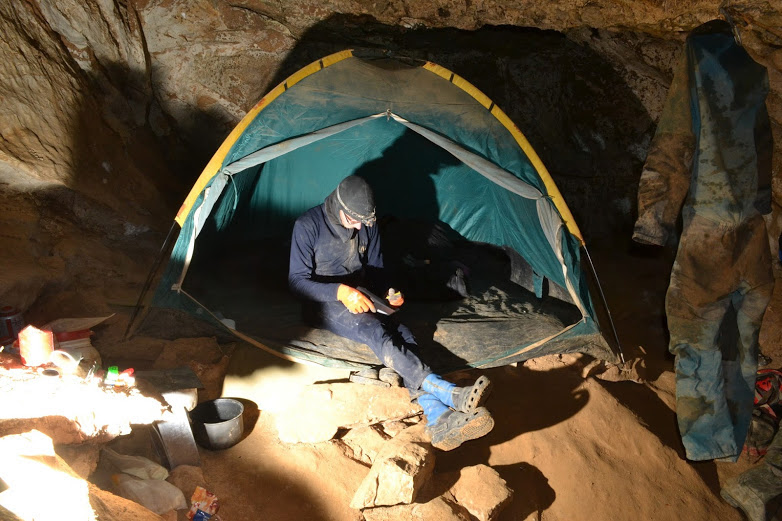
\includegraphics[width=\textwidth]{campxray.jpg}
\caption{Writing in the log book at Camp X-Ray --- Rhys Tyers}
\label{Camp X-Ray}
\end{figure}

We drifted to sleep. People will go on about how they woke up in complete darkness and how they were assailed by all sorts of strange oppressive thoughts. A hungry stomach, and somewhat sore back saw to it that I stayed focused as I woke up. Living underground came quite naturally as I put a pan on the fire, coming and going in the ageing homemade slippers. A meal was soon ready, and we wolfed it down. Then I had a look at the state of my fleece undersuit. It was mildly damp. Same for the gloves and the wetsocks. 'Carry on we must' I thought, sighing slightly. Rhys must have heard for he exclaimed 'now for the worst part of your daily routine: putting wetsock one and wetsock two'. In truth those two socks, hanging in the darkness, trying their best to dry off but ultimately failing made quite sorry sight. Five minutes later though, with welly boots on, blood started circulating and warming them a bit, until we were as ready as we were likely to get, so we set off for the southern reaches of the System.

We entered the deep, dark cleft at the bottom of Zimmer and soon descended a very non-enticing muddy pitch. Some three or four challenging (for a fresher) rebelays later, I was swinging at the bottom hang to land on a balcony. The pitch had intercepted a wide horizontal passage. Rhys pointed at the dark space beyond the pitch, at the other window saying:' this is the way to the connection'. His eyes were a little brighter it seemed, but I said nothing at the time. Rhys was a very helpful guide as he described every junction we faced. 'Put your feet here', 'look around so you remember which way to go on the way out' 'If you go that way you walk for fifteen minutes until you hit a dead end' etc? We found another very muddy pitch on the way, Stuck in Paradise it was called. Apparently it was far better now than when first discovered. I made a mental note to find a bypass as one of the expedition's aims. It is very slippery, and quite unstable I found out later ( that's another story). Some of the rigging is very tight and I spent a good ten minutes trying to recover from a breaking carabiner trying to change places with by descender. When footholds are scarce, hanging rebelays are lonesome places at the best of times. But seven hundred metres down, with nothing but mud to hang on to, they are objectively challenging. Cursing and muttering I finally freed myself with a waning arm strength.

Down the pitch we found Hawaii, and a Darren drum, mess tin and a few lengths of red '9 mil rope'. Time for a little break and history lesson. There, Tetley and Sam had been assailed by a non-troglobitic creature, mammal, as large as a bear, as cunning as a fox, or as adorable as a cat depending on the stories. Fighting for their lives, they had later brought back some food to offer up to the cave gods on the Hawaii altar. And hours later, the gods had taken their due (or hid it under a rock). 

I had a look at the Darren drum they had left there. This part of the cave is quite dry. It is at least 500m from any running water in all directions, and barred by an incredibly muddy pitch to the west, a knee killer crawl to the east. The southern passage is the longest, with various crawls and squeezes to get past. I started to get an understanding of the logistics involved in such deep and hostile environments.


I was less impressed when I unscrewed the lid though: a brown layer of silt had settled out of suspension at the bottom, over 11 months, but as I moved the keg, it all mixed again. 'Must be gritty then, I'll be sure to bring water of my own if I come by next time', I thought to myself. Luckily I had a bottle with me, and it was half full.

Time pressed, so we carried on towards the southern reaches. Rhys looked around, and showed the uninviting offshoot to Hash. 'The anthropomorphic section ends in a dogleg even Clare was scared of...' That said it all. We carried on, until we found the boulder choke at the end of Lost Miles. Off came the SRT kit, and we squeezed through. There began Atlantis. After a time we hit a junction. To the left, the continuation of our journey. The stalactites were there, as I had been promised. I was also told to be very careful, they were one of the rare formations in Migovec. In that region of the cave we were on the look out  for Dave had warned us about a passage leading off to 'We're Not Alone' to our left. It was an obvious beckoning darkhole when coming from the pushing front, less so on the way there, by we looked at the blackness beyond, trying to fathom the distance the passage went, to little avail. We probably just needed to walk the few metres, but instead we pressed on. Down, further south still. The ceiling then started to come down, until after a little sandy and pebbly crawl led to more opening. And then the boulder choke.

With a little hesitation about what where the lead actually was, the flat out crawl was negotiated. After a sharp bend it opened up and turned to walking phreatic passage with a strong draught. One large ledge protruded from each side, providing a path 1.5 metre from the ground with mud ripples and other multiple mud formations. It continued for 20 metres until a shadowy alcove appeared to the left, and a pit to the right. Climbing into the alcove the passage became tunnel shaped and sandy until it hit a junction 15 metres later. The lead was pushed northward and upwind and again a pit appeared on the right before a turn to the left. It seemed never to end and every pit, or junction opened more possibilities. I was thrilled. It was, by any standards a great find for a first pushing trip, because we'd left more leads than we started with, and good leads they were too. I started thinking about finding our way back, perhaps I was far too keen at that point, and started building a cairn with elongate pebbles showing the way back.

Rhys on the other hand left little notes with helpful messages and tips on such as 'pitch undescended as of 21st Sept and so on. Having turned left from the pitch head (we had no rope), there was an awkward pit traverse. I free climbed down to check for any leads, and I believe there is one. Instead, we chose the more obvious passage after the pit. Whenever it seemed to close down there was an obscure way on. We passed two sandy circular chambers separated by constrictions. This led to a larger chamber with a boulder floor sloping toward the north, with bit of a free climb to go down. At the western end the draught disappeared through another constriction from which the trickle of water could be heard. The passage ended 10 metres later at the foot of a 5 metre high waterfall. The water pooled at the bottom before flowing eastward through the boulders. A way on could be seen from there, underneath the pile of boulders, but it wasn't checked this year. Content with the amount of passage found so far we decided to start the surveying of the chamber. Since we were both presidents, (I was president elect at the time) we settled upon the name Sic Semper Tyrannis. This literally translates as 'This is what happens to tyrants''. My body temperature decided to fall at that point, and this part wasn't as entertaining as discovering had been. Nonetheless seeing that leg after leg length was indeed building up, we started to grasp the size of the passage, and its rough shape. We had gone further south still, maybe as south as caving in Migovec goes. Back in the large boulder chamber, we had a brew.

'You see this window at the top of the boulder slope', Rhys pointed out to me. I say we have a look and if it doesn't go, we look at the large junction and follow it downwind.' So I scrambled up the slope, and through the narrow opening...to emerge into a huge chamber. I bit back an exclamation, simply saying 'You should go up there... definitely'. I stood and had a panoramic look. It was the biggest deep space I'd been in so far. There was a white lip of rock, sitting close to the ceiling at the opposite end, and a steep rubble and boulder slope in between. I dare not go further up without supervision instead gorged myself on the view. The slab of white rock really looked like teeth guarding the open mouth at the top.
With my spot light on, I tried to peek at the space beyond. Rhys stood behind me, and we shared a look of contentment at the find. It would be 'easy bolt climbing', being more of an inclined chamber than an aven. Still we had a look on the slope, and two openings at the bottom led to a small cozy chamber with a little waterfall and clean grey white limestone. It pooled at the bottom and went somewhere. We immediately thought about the waterfall chamber below. We surveyed this, named the chamber 'Helm's Deep' for the wall of white limestone guarding the way on (and also the fact that we were at -800m and any Middle Earth inspired name had a nice ring to it). The source of the water could not followed for long though because it emerged from a sharp and narrow rift.

More than content, we surveyed this short leg and started the long way home. Home, a surprising thought ! Camp X-Ray was a good as any home now. 'Now you feel you are deep and far from the exit don't you ?' 'Yes Rhys'. It was a long and hard way back, but we made it back shortly after 8 o'clock. Once again I blessed the warmth of the gritty tea...



\subsubsection{Digging in B10}
'so this is a digging tray?' I exclaimed. The bivi was crowded in the late morning. Rhys and Dave had gone down to the underground camp to push the large junction of Sic Semper Tyrannis, Will French and James had also gone down, although they were pushing a streamway closer to X-Ray. With time on my hands, I volunteered to help out with the digging of B10, led by Dave Wilson and Pete Hambly. Fiona wanted to come too to spot the entrance and help out with disposing of the dug out rocks. The digging tray was a jerrican whose side was cut out tied to a rope on both ends for easier handling in tight passages. Dave packed a small spade, two crowbars, one large, one smaller and some comf. I was excited to see the digging techniques put in action.

The sky was heavy with cloud, and it seemed for a time as if we'd escape the rain altogether if we quickened the pace to the entrance. On the Kuk path we headed north, until a large grassy valley on the left leads to the plateau's edge. On the left a large sign painted on the rock indicated we'd reached the cave entrance. A few metres on, an obvious pit was marked with the sign 'N4'.  We gathered around the pit and looked at the nodules that protruded and seemed provide a safe free climb route. Dave put his foot on the first but frowned instantly, gave it a mighty whack with the back of the boot and the whole lump fo rock tumbled down. Now that the climb was much more daunting, no foolish explorer would risk climbing without a rope.

\begin{figure}[h]
\centering
\includegraphics[width=\textwidth]{Atlantix.jpg}
\caption{The stalactites of Atlantis passage --- Rhys Tyers}
\label{stalactites Atlantis}
\end{figure}

The entrance to B10 led away from the cliff, at a steady angle downwards. It began as a spacious crawl, with red mud at the bottom, dark grey crystalline limestone on top. Soon the passage closed down to a squeeze only Dave Kp had attempted the year before. With both arms tucked underneath my body at the tightest point, I shimmied down and went through to the very small chamber (here the term is loosely applied, the passage is just large enough that a U-turn manoeuvre is possible). Beyond, the passage was tight and very low, but it was mostly made of cobbles with a muddy matrix holding them together. 

I turned around and asked for the tray, the comf and the digging instruments. While Pete and Dave started shuffling rocks from the entrance passage before the constriction to make the access easier, I attacked the squeeze from the other size. After lining the floor with a roll mat I lay insulated from the ground and started the work. This involved using the leverage from the crowbar to pop cobbles out of their mud matrix, and filling the tray. After an 'Ok' the tray would disappear, pulled by the other party, and after another vocal signal, I would pull on my end of the rope to bring it back, and fill it again. And again. 

This was hard work, and soon I longed to see the outside again. Near the entrance, the walls were dripping, and some of the water was beginning to find its way down the small chamber. After an hour or two work, the squeeze was perfectly manageable, but further enlargement would also make it easier to dig. Positive feedback!

\subsubsection{Back to Sic Semper Tyrannis}
My second underground camping trip this year took me back to the end of the Atlantis passage, where with the help of Samuel Page a further 25 metres of passage was found in a multi-level rift. We had booked two nights at camp, and descended early to have an extra day of pushing. That is might be a tad ambitious dawned on us upon arrival at X-Ray. Rhys and Dave, who'd pushed there the day before were in for a tourist trip in the deep places of Migovec, so instead of pushing south, we visited the Fridge, saw the joys of Big Rock Candy Mountain for the first time and examined the dig at Kokaine Lab. It is said it might connect with another passage off the Atlantis branch. Such a loop would be indeed a great tour of the system.

We set off on the morrow for our pushing trip in Sic Semper Tyrannis, following Rhys's guide notes at every ambiguous junction. After three hours at a steady pace, with the mud madness of Stuck in Paradise behind us, and the flat out crawl in front I set foot again on Sic Semper Tyrannis.
First of all, I wanted to look back at the large chamber, and seek a way past the white wall at the top of the rubble and boulder slope. Sam quickly took refuge out of the way as I sent an avalanche of 'particles' hurling down. Fortunately a small alcove provided a safe haven for him. As I reached the bottom of the white rock slab I realised how precarious my situation was, and without further ado climbed back down.

We settled for an easier lead, Jericho, that had been discovered downwind of the large junction by Rhys and Dave Kp the day earlier. The passage started to slope upwards, gently at first, until the way on was either through a squeeze or an aven. We'd spoken with the pair about it, and decided that I should go through the squeeze, then rig the aven from above, to provide an 'all sizes welcome' entrance to the pushing front. I was thrilled as this was about to test my ability to bolt and rig without supervision.

I squeezed passably well, then climbed and examined the pitch head to be. The rock was poor, the hammer heavy, the bolts are unsafe and placed at the worst possible spot. It urgently needed rebolting, even though Sam was kind enough to praise my effort twice by ascending and then descending without any hesitation.

Then we bridged the rift, up and up until it became frankly scary. This I understood must have been the end of exploration. With a bit more bridging I was up and away, in a higher level of the rift, very muddy and extending both north and south. This section of the rift should be made safe by dropping a rope, approximately 25 metres are needed from the top. The draught was chilly there, and we decided not to stay long therefore we explored both ways leading from the top of the climb. Back north quickly choked, whereas carrying on south leads to a small pit. My guts betrayed me at the sight of this and we turned round with a meagre 25 metres of passage. Nothing ventured, nothing gained. The rift continues... After the chill of Jericho, we made it back to the large boulder chamber and had a soup at the same spot as the previous time I'd been. I realised I had no water bottle, so filled the little pan directly at the waterfall chamber. The warmth slowly radiated in our limbs, lifting our spirits, and setting us up for the journey back.

Arriving at the beginning of Lost Miles, after the boulder choke, I began to feel very dehydrated, so cursed for the lack of my battered bottle. We then reached Hawaii, and started feeling very uncomfortable. That is when I saw the Darren drum I knew was filled with silty water...

This however wasn't the end of the troubles as halfway up Stuck in Paradise, I grabbed... (I know it's happened to everyone) what looked like a stable nodule. To my horror, a beast of a boulder started coming loose, and slid a few inches down the slope. I froze, until it stopped. Carefully manoeuvring around it I called with a rather shrill voice 'sAM....', 'Yes ?', 'I've just dislodged a BIG boulder, be careful around the next rebelay !.... 'Okay'. With little relief I started ascending, half expecting the boulder to suddenly disappear in the blackness below. I passed the next anchor, and then the next. I was breathing more calml... BAOOOM.
'sAM !'...'Yes ?' A muffled voice answered. 'Was that the boulder ?' 'Yes'. 'see you at the top then'...' OK'.


\subsubsection{Five days under}
The final trip, over 98 hours long was by far the most demanding but it taught me the value of perseverance at one pushing front. Since I had never pushed at the same front in one trip, to go back to the same passage four times in a row was undoubtedly trying my commitment to the caving cause. In hindsight, it appears to be the only way any significant progress could have been made because it meant we were the only pair to know the ground, which enabled us to push more efficiently.

After the small squeeze, I found a small sign by Rhys and a length of tatty rope indicating the way on. I looked at the little hole in the thin rock wall, downwind and to the left lead towards the Red Baron, and further still the distant blackness of Atlantis. Right however... A square of paper written by Tetley indicated the Kamikaze 'lead'.  Aileen and I, full of resolve made our way through the sandy walking passage.

The ceiling quickly dropped, but on we went, until a point where a natural bench beckoned for a rest. Aileen proposed we put the SRT kit in one of the bags as the crawling became unpleasant. I obliged, and we were on our way minutes later. The walls were covered in red dust, it was quite spectacular. Halfway down the crawl there is a sharp bend at a small pit, and after it began the bedding plane crawl. There was an offshoot to the left. My memory of it is that of a uninviting lead. It may be because the ceiling is markedly lower than upwards, and upwards is tight. In fact, a size 10 foot can use touch both ceiling and floor of the bedding plane with heel and toe, and it is a remarkably good technique to move up. I have experimented pulling and pushing the tacklesacks but haven't found any preference, in fact it is just annoyingly tight. After the plane, the passage was followed upwards through little ponds and small 'nipple' crystals. A little spearhead of a rock indicated the end of exploration with 'PSS Kamikaze 1 2010 Dave Wilson and James Kirkpatrick, next to the blockage.
There was space both below and above the boulder and the gentle gurgling of a waterfall could be heard beyond. It was certainly a little way from the squeeze though, or else the water had moved since the first exploration of the passage. When Tetley and Johnny came back to investigate the leads in 2011, a year renowned for the vast amounts of water shed on the plateau it is likely that the passage was in flood at the time. It turned out Aileen and I on the other hand had left while cavers on the surface gorged themselves on a long spell of sunshine and so the water levels were low.

Moving the boulder, Dave reckoned might just be possible with the aid of chisel and crowbar, provided there was space lower down the plane. It turned out the cross section of the boulder was a lozenge. The tapering edges being readily 'amputated' through mad bashing, we gained more scope for movement, and inch by inch, the blockage slid towards us, until enough room was made to the upper left corner.

In order to get past the FORCEPS towards the exploration front, one simply has to shimmy upwards, and provided one's legs are neither too long nor too thick, one has to move them one at a time over the tapered edge of the boulder and then slide back down the other side, feet first. It is advised to carry all tackle through the squeeze whilst people are on either side ! The way back to camp is miles more fun, as you simply can simply dive head first through the squeeze.

Using the technique described above, I slid on the shores of the unknown, with Aileen close behind. The chamber appeared to be of small dimensions, with some degree of boulder collapse in the centre. To the right ( north east) a window overlooked a dribble of water cascading down the opposite way.

We cursed, for the lack of rope and time meant we had to turn there for the day and head back to camp. We still had three more days booked, and it looked increasingly like we might be staying at this one pushing front. So much for planning a 'grand tour of the system', the thrill of exploration was beginning to take root. Deciding not to survey this 10x4 chamber, we headed back? after Aileen, using a sling as belay perched herself atop the pitch head to have a better look. The cascade needed rigging, and it looked like it was closing down?

We made it back to camp at a decent hour. Some well deserved 'secrets of the forest and wine' later, with the stoves bubbling merrily and more tea on the go, Gergely and Izi started to try and fettle Aileen's ceased central maillon (note: always choose steel over aluminium alloy for the thread is much the sturdier). It didn't work out, but a hidden cache of bio pork from Erik's uncle farm was discovered and was quickly cut into cubes to be had with local cheese and bread brought from the surface. It was indeed a feast, and Aileen was undoubtedly right in saying that the quality of underground food had to be even higher than on the surface to counterbalance the lack of comfort.

The second day, we were up early, and soon on our way to Kamikaze. Back at the front, and sweating from the crawl, Aileen started bolting the pitch head. The rock was loose, and it took the best part of an hour to get one bolt in. We had no spanner (my fault, never to be repeated) and as a result, any dirt in the thread that would impinge the screwing of the hanger was fatal to the attempt. However, in the end the pitch was rigged, and well at that dare I say. There is a deviation from a flake 3 metres down to keep out of the cascade, and then a 4 metre hang, rather wet at the bottom. The passage indeed closed down after the little pool, with the water dribbling away into a small rift. It was however passable, and the way is between two obvious ledges protruding. It is dry. Squeezing upwards after 3 metres leads to a roomier space, with boulders as a false floor.

The pitch head was obvious, and so were the boulders threatening to obstruct it. So while I cut the rope from the other pitch and cauterised the wound, Aileen started gardening. It all went to plan, we could see the drop afterwards, with the water coming from the side. It all went to plan, until a TV (not an idiom we're likely to use for much longer, TV's are all flat and thin now) sized boulder slid down the pitch head and got jammed there. We had no pitch head left !

We were quite annoyed at that to say the least. We did not give up quite yet, although the thought occurred quite frequently in my mind. It is interesting how on the surface we commit ourselves to more than what we are really up to in the cold and lonesome places that are pushing fronts. We had booked four nights at underground camp, and we were going to break through. After all we had done it the day before.

Recalling the way I'd freed a boulder in Jailbreak before, and the training in Yorkshire the previous winter, we decided to pulley-jammer the rock out. It had worked before I knew, but the rock here was a) jammed, b) quite a bit heavier c) very close to the pulley, therefore hard to manoeuvre. Finally due to the lack of space, using my person as a counterweight was out of the question. Remained the strength of my quad muscles...

The rock remained jammed, despite our best efforts. What we needed was what we had on the eve to free the first blockage: chisel and crowbar. With that in mind, we started the survey of the passage we'd found so far. We had to find a name first. We had dug our way in the new passage, so thoughts of the great escape were never far. I knew we used inkscape to draw the survey so I proposed 'the great inkscape', a very mediocre play on words. To which Aileen replied 'that's a pun too far'. There we had it I thought, so we settled on 'a Pun too Far', with an allusion to another classic war film. As we finished the survey, the hour was growing late so we trudged back to camp.

Back there, we had a change of company: Rhys and Sarah had come down to do some easy pushing. We shared a lively supper before drifting to sleep.
Being early birds again, we cooked breakfast under Rhys's unimpressed eye. 'They have yet to understand the principle of camp faff' is what I believe was written down in the Underground Logbook. Oblivious to the disapproving gaze, we set off a third time. We had chisel and crowbar at the ready, and would crack this boulder open with a mailed fist...
We managed the crawl ever more swiftly, as every turn and angular pebble became more familiar, squeezed past the Forceps with ease, descended the cascade pitch, wriggled through the rift, and emerged on the false floor. Without wasting any moment, we started hammering at the rock. 

'If we could get rid of that nodule, then maybe,..., put the crowbar here.... heave.... hammer.... push, no pull. What about this nodule ? Chisel... heave now, it's moving ! HEAVE?' 
To no avail. The boulder was well and truly jammed. It was marginally reduced in size, and rock powder was in the air.

I bit back a sigh. I was warm now and panting from the effort. The dribble of the water below was more tantalising by the instant. In a stroke of genius, Aileen started 'If we could secure the boulder, I mean it IS jammed, there might be enough space to squeeze underneath, all we'd have to do is ? more chiseling to enlarge the pitch head'.
I knew this pitch head would be awkward whatever the outcome: very tight, and with a spear of rock about a metre underneath. But I started chiseling madly at the rock. Now that the plan we had seemed to be functional, the thrill of exploration drove my hand down, and down, and down again with a renewed energy. In minutes, a few good sized nodules had been chipped away. In the end, it needed a few more furious blows before Aileen's helmet disappeared underneath.

I eagerly followed, managed the squeeze by hanging my ascending gear from the long cow's tails. I was elated when my feet touched the floor. There we were, back in the little stream and the chase for the lead was on.

The rift we then followed is very much controlled by an oblique fault. We followed the passage down for a few turns until it seemed to close down again. However, shimmying upwards again lead to an opening... is that the splashing of water droplets down a cascade ? The awkward crawl led to yet another pitch head!
And this one was larger than the two small drops we'd found during the earlier days. Again, muttering a curse, we realised that we were lacking rope to descend it. This drop however represented the first big opening of the passage after the breakthrough, so we shook hands on the discovery, and surveyed all the way back to the jammed boulder.

Seeing as we hoped to bottom the pitch on the morrow and what we had found amounted to a few tens of metres, we carried on with the name A Pun Too Far. We surveyed the rift, and at the pitch head, thought of a name for the very tight pitch head. We had chiseled away most of the rock and Phydias's folly seemed appropriate.
For a third time, we went back to camp. We met Rhys and Sarah there. From what I heard, they'd pushed something horrible. Worse they'd taken the camera we had only to take photographs of a thick vegetable soup. That's another story altogether. They would be going up on the morrow. We wouldn't yet, we had a pitch to bottom...
And so we did, by noon on the fourth pushing trip, we were down the pitch. To our dismay it all closed down again, but we followed the rift, free climbing a 2 metre drop into a small pool, down more rift. It didn't end, there was always more. It twisted and twisted until again it opened up, into a circular seven metre drop. It was getting late on the last trip we intended to do, so we turned back then, leaving a storming lead for the following year. Before leaving the limit of the exploration, we has a small photo session.

The fourth morning was the worst, knowing there was no escaping the 550metre ascent. The long stay underground was wearing on me know, and the long pitches finished me. My footloop snapped in the Urinal Series, this setback gave a little rest, and with Aileen's spare dyneema footloop, I raced upwards. Depth clocked down quickly, and all too soon the final squeezes were behind. One last scramble up the scree slope. Daylight, warmth and a can of beer !

\subsubsection{Epilogue}
'Hey ho!' Silence. 'does it go ?', 'do you want some tea?', 'yes', 'cow ?', 'no'...
'Yes the cave goes, it always goes, the mountain is hollow after all.' 'shall we enter the survey data now ?', 'Of course'. And little by little the 150 metres or so of passage are added to the grand survey. What a joy to see four days worth of work take shape before one's eyes ! Where does it head to? Is it blank mountain ? As ever we raise more questions than we actually answer.

There lies the thrill of exploration: more people have been to the Moon than in the passage we found. Tomorrow though is the expedition D-Day. This was the final caving day when we will put the cave to sleep for another year by packing up camp X- Ray and finally head down to Tolmin the nearby town in the valley before the long journey home. 

\begin{figure}[h]
\centering
\includegraphics[width=\textwidth]{The plateau.jpg}
\caption{The Migovec Plateau, looking south}
\label{the plateau}
\end{figure}






\chapter{2015 - Pivo moz} 
\begin{flushright}
\huge \it Beer Man
\end{flushright}

\section{Coincidence Cave}
 \begin{verse}
Jack Hare
\end{verse}

Rhys and James returned to the bivi, buzzing with excitement about the new passage they had found, Jetstream. We entered the survey data into the OLPC, and found that the passage ran due south, towards the face of Mig. We could hardly have been more excited - the prospect of a lower entrance seemed clear, and the glory would clearly go to the ones who found it. With no prospect of going underground, I resolved to search on the surface, and on the next day, put my plan into action.

I spent some time learning how to use the survey software, and this provided a coordinate for the location directly above the end of Jetstream. It seemed reasonable to begin our search for the lower entrance there. After a great deal of anguish dealing with the conversion between Slovenian coordinates and the more commonly supported UTM, I realised that all I really needed was a bearing and direction from something we already had a UTM coordinate for, namely Gardeners? World. Our torturous calculations are included in the bivi log book. Spookily, the end of Jetstream is absolutely due south of Gardener?s world. I entered the coordinates of our prize into a GPS, and Rhys and I set off above ground to find it.

The day was ridiculously hot, and we had not brought enough water. We dropped down the east side of Mig towards Gardeners? World. Instead of following Janet?s path to Razor, we decided to cut across a thicket of dwarf pine. I recommend against this route - almost anything is quicker than pushing through dwarf pine, and we became hot, sweaty and dehydrated in no time.

Eventually, we regained Janet?s path, and followed it round to a junction with several real paths. We took the western route, back towards Kal - we knew we were still too far north, but we weren?t aware of another path, and we decided we could always drop off the path to the south when we got to the right location.

As we walked, it became clear that the mountain was steeply sloping, and that it would be difficult to actually leave the path to go looking. We continued along, hoping for a break in the trees, and as we arrived at the point due north of our goal, we came across a canyon. This dry canyon runs directly south from the face of Migovec, bisecting the path. It is not very deep, more of a scoured river bed, but it runs down over steep terrain. At the bottom of the canyon we could clearly see Ravne.

We were hundreds of meters too far north, but the canyon was incredible - Rhys didn?t remember anyone mentioning it before, though it was hardly hidden! We started to down climb it, scrambling over boulders and down short cascades for a few tens of metres. Soon it became too steep, and we worried we wouldn?t be able to climb back up, so we retreated to the path.

At the point, we recalled a path lower down that followed a parallel path, contouring along the cliff face. It splits off just before the final forest that precedes Kal. So we headed to Kal, stocked up on water and apple sours, and the continued down into the blissful shade. Very soon we refound the canyon, and could see it extend far north to the face of Migovec and far south to Kal. We were very excited, and dumped out light bags to climb up the dry canyon. The free climbing seemed sketchy this first time, and I almost walked into a web with a huge spider waiting to devour me. 

After checking a few obvious holes, we hit the jackpot around 40 metres up. In a vertical section of the canyon was a dark hole, just body sized, pushing horizontally into the rock. It smelled damp and the air coming out was cold. Sticking my head inside, the size of the draught was obvious. It was clear that this was a strong lead, and Rhys and I were very excited.

We made our way back to the path, resolving to look south down the canyon before heading back to the bivi to pick up digging supplies. As we drank our water and rested, we heard familiar voices approaching along the path. It was Dave W, Dewi and Pete, this year known as the Three Wise Men. They?d been hunting for the lower entrance for the past two weeks, and had been dragged up a terrible route by Pete?s GPS. We explained what we?d found, and Pete confidently announced that he had already GPS tagged this cave, but that it didn?t go.

Dewi was unconvinced, and we led him up to the cave. He became immediately excited, screaming insults at Pete and pulling out huge chunks of rock with his bare hands. An impromptu digging party occurred, but without our kit we didn?t make much progress. It did become clear that this was going to be a big job, and no easy break through. After some debate, we agreed to name the lead ?Coincidence Cave? in honour of the great coincidence that occurred. The name that Rhys and I proposed, ?Seren-fucking-dipity Cave? was not considered adequately solemn.

Over the next few days I returned to the dig, commuting from the Bivi with my caving kit. These were long, tiring days, and I joined with Dewi, Dave and Pete in digging shifts of around half an hour. Progress was slow and tedious, but I learned a lot about digging. At the deepest limits of the dig, a loud, low rumbling sound seemed to come from the passage ahead. At first I assumed it was thunder, but when I got out of the dig, I found that there hadn?t been any. This noise would be consistent with a waterfall.

Jim Evans joined us on one day and showed a great deal of enthusiasm. On my last day on Mig, I waited with Katy Morgan for a smoke signal that Tanguy and Rhys were going to set, but we saw nothing. Later it transpired that they hadn?t set the smoke signal, so that makes sense.

Further exploration of Jetstream found a passage that extends even further south than Coincidence Cave, and deeper underground. If Coincidence Cave is a lower entrance to the system, as I believe, then it enters into passages at a higher level than those we can push from underground. This alone is enough to tempt me back to the dig.

\section{Deep camping at Red Cow}
 \begin{verse}
Jarvist Frost
\end{verse}

\section{Hundreds of metres of (mostly) walking passage} 
 \begin{verse}
Tanguy Racine
\end{verse}
\subsubsection{The finding of Meridian Way} 

The quest of finding a lower entrance to the system is without any doubt a noble one and hasn't been completed as I write these lines. The Jetstream extension of the system was spearing south, well away from the main tangle of passages that make up Sysmig. Less than 400m to the surface, southwards and upwards, the chances of ending the push by popping out onto the sunlit forest floor were as good as any. In fact, they were better than that: the serendipitous discovery of Coincidence Cave earlier in the week had revived the belief that the entrance might exist. A draughting hole on the surface, the alignment of a large surface canyon with the underground passage, what are the odds' 

Rhys and I checked in at camp X-Ray for three nights and two pushing days. The ambitious plan was to set off smokers at the pushing front, while a party on the surface waited for the red smoke to come out thus proving the connectedness of the passage. This would bring us much needed closure.
	. 
After an early start, Rhys and I set off  from camp, along the now familiar Kamikaze extensions, the long silent passages of Atlantis. To our left, the offshoot of We're Not Alone beckoned. With the limit of exploration so close, we could not help but have a look at it, to assess the feasibility of pushing the lead. The passage first trended east and bent to the south sharply before turning into a flat cleanwashed crawl. With the ceiling coming to meet the floor to a tight, awkward flat out squeeze, it was no wonder the lead had been left unpushed. Passage could be seen continuing beyond, but we left it at what it was: a lead for thin people. 

It was almost eleven o'clock, we had been caving at a good pace, and the front was half an hour away. We pressed on, past the boulder field leading to Sic Semper Tyrannis, along passages named and trodden since the previous year only. At the main junction to Jericho, we turned left, upwind, up the rift. I passed the down climb to Squidgy Goodness where the corpse of the Creature was, and up the ropes Gergely had rigged in 2014. Rhys disappeared down the next pitch, which was the beginning of Jetstream and showed me the way up the climbs. 

At the very apex of surveyed passage of Jetstream, the rift split into two routes. One was continuing directly upwards in the same fashion as the ten metre pit we'd just free climbed. The convenient ledges that had brought us this far disappeared quickly and it was deemed unsafe without a rope. Glory would have to wait. Instead, we slid down the slanting rift continuation, down the scree slope to a boulder choke. When faced with the pushing front, crowbar in hand and with a clear idea of what was to be done, a smile crept on my face: that was precisely what I'd signed up for, thrilled by the countless possibilities of what lay beyond!

I levered a block of limestone out of the choke, then pushed two others to the side, and the way on was clear. I wriggled forward, both hands forward, getting a grip on the boulders on the other side and sat, looking, silent. Rhys followed quickly.

Grinning at the continuation, we stepped off to find the lower entrance. For about 30m the dream was on because the cave didn't change nature: it remained an unstable chossy bedding plane descent. I heard Rhys commenting on the lack of easy walking passage.

Almost as an answer to our expectations,  the passage opened up almost instantly into a walking, dry, vadose passage and better still, led to a junction ! Rhys stepped to the right, I to the left. The passage on the left twisted down and up before resuming its southern course,  but the fault control, pervasive in that part of the cave meant it was going down, ever so slightly towards the west. 'Of course!' I thought.The faults were dipping west, and we were locked on their plane. Occasionally I would point out to Rhys where the fault planes were exposed, they were beautifully smooth.

When the passage wormed it's way to the top of a sloping pitch, we knew it was almost a game over for us. We were too deep, or not far enough south to intercept the surface. Descending the pitch meant we had to find more horizontal distance! Still, we decided to descent, first by free climbing the 55∞ slope, using the various ledges covered by white sand. About 5 metres down, the slope increased and it dawned on us that we would have to bolt it. 

Having left our rope and bolting kit at the start of the squeeze, we doubled back to retrieve them and set about driving the anchors for a Y-hang. I put in the first one, far above the pitch head as it was easier for a left-handed person. Rhys put in the other, and rigged his descender. Down he went until he reached the stopper knot. The end of the pitch was in sight, but the rope was a good ten metres short. It would also need to be deviated.
 
We considered our options: there was rope at the junction at the start of Jericho, but the horror of Jetstream (Penitence like crawl, loose climb, muddy slope etc') had to be passed again and again.  As it was approaching two o'clock, we resolved to abandon the plan to set off the smokers and  instead to simply reach the bottom of the pitch and see what was there.

At Jericho junction, after a soupy-fishy-couscous mix, we retrieved the longer rope and turned back towards the pushing front. At the pitch head, I descended slowly, watching the rope carefully to avoid rub points on the various ledges. I had put a deviation two thirds of the way down which ended up swallowing 5 metres of green tape. This done, my feet touched the floor once more on virgin passage. I stayed silent as Rhys descended.
 
Below the pitch (measured to 25m at 55°ˆž), the passage opened up to intersect a 5x2m horizontal passage trending south. This was our way to the surface! Then followed the best minutes of exploration along a seemingly endless horizontal passage. I thought of Atlantis, of Friendship Gallery, of all the reports, stories, tales even, of glorious easy walking passage and felt immense pride in walking alongside Rhys in this gallery. 

Along the way, we noted several interesting features: bits of hair, excrements, scratchmarks, bones! It was all there, the proof that mammals of some sort have been here before. To the best of my knowledge, the Creature is trogloxene, it's presence only explained by the ease with which it could move from a lower entrance to this passage. Indeed, the fact that one could have made it's way to Hawaii doesn't seem as remotely incredible as it once did. The majority of passage from the end of our gallery to Hawaii is simply horizontal! 

We turned round and surveyed the 'Meridian Way' when a boulder choke prevented the easy walking. The passage goes on - to the lower exit - it must! Back at the pitch base, the passage also disappeared into darkness towards the north. Another long gallery' We would have to wait for another team to explore this one, for us this was the beginning of a long survey, and an even longer return journey.


\subsubsection{Pushing our Luck above Cuckoo's Nest}

We'd overslept a lot I decided as I saw that it was already past ten o'clock. It did not surprise me, since we'd only come back from Meridian Way just before midnight. Then we'd collapsed into bed.
 In the darkness of the tent I sat upright in the snug sleeping bag, furry hat on. My breath turned to a silvery mist by the light of my headtorch. The fairy lights had dimmed so much I could hardly make them out. I left the comfort and warmth of the Nitestar 450, put on the largest crocks I could find, and lit the church candles. One, two, three dancing lights. 

'Where are we going to push then'' I asked Rhys, whilst tucking into a rich soupy couscous mix. 
'I know of a lead Clare pushed in 2013, up Cuckoo's Nest' he replied. 
'I've never been down that way. How do you get to the passage' Is it past the traverse at the top of Big Rock Candy Mountain''
'Yeah, that's it, you traverse and then drop into a chamber. There'll be a rope on your right, the one from Euphrates. It's a grim bit of cave, which is why no one's ever gone back to retrieve the rope after surveying. It connects back to Xanadon't and the hole in Friendship Gallery.'
'Fascinating, so fairly close to camp then. Shall we' I'm going to put our call out as 7pm then'. 

Half an hour later, we left camp, along Friendship Gallery, towards the head of Big Rock. There we kept to the right, traversed on the muddy pitch head, until a short succession of small hangs brought us into a chamber overlooking the massive drop. After a small climb down, we followed a sinuous muddy rift until we had to climb up again unsing a greasy in situ rope. From then on, the rumble of flowing water could be heard distinctly, and we soon came upon a fork in the passage, with the way to Straight Jacket and Rejuvenation Rift to our right. The way on to the end of Cuckoo's nest was to the left, with the passage descending slightly until we reached the water at the bottom of the rift.

Past a few meanders, the rift widened to an oval shape and a cascade three metres high draped the far wall. A PSS was left underneath a egg like pure white limeston cobble: Cuckoo's Nest station 3. Rhys and I contemplated the pushing front. The only viable way on was up, and could be reached by bridging our way up, away from the water. Several ledges were seen to protrude, giving steady footholds about two and a half metres from the floor. Feet and back against the scalloped walls, Rhys  climbed up gracefully and I followed.

At the first ledge I started removing the majority of loose rocks I could reach, while Rhys gained more height. Ledge by ledge we climbed until we reached the top of the traverse, dry, muddy, and loose. There we steadily traversed in the upstream direction, until we dropped into the streamway again. We were faced with a similar second climb. Further traverse enabled us to gain the top of third cascade, after which we continued almost a stream level on a meandering rift heading steadily southward.

Our progress was not hampered by any further climbs or constrictions, and soon I lost count of the twists and turns. We arrived a boulder collapse. Navigating our way in the vertical maze we eventually reached the roof again, but to our surprise, a flat out crawl lead off back in the opposite direction. Instead of following it we negotiated the way past the collapse, and regained the stream. From then on, the rift enlarged particularly on the occasion of three meanders, where the base was very much wider, the stream lazier and where sediments had deposited on the shelves: granules and small pebbles of white limestone and black haematite. This was a delightful sight, the finest photogenic cave sediments I'd seen on Mig! 

After the meanders, the rift resumed its course and after a further collapse Rhys and I called it day. This was more than enough rift to survey. Doubling back to the start of the passage to get survey paper and instruments, we tried to gauge the length of our find. With the 350m discovered a day earlier at Meridian Way, would we reach the 500m of passage found in one camping trip'

As I took the survey notebook and pencil, I stuffed my gloves inside my oversuit, and we started the survey. After the climbs, we started the meanders. As I sat, writing down the lengths and angles Rhys dictated the gloves fell down to my navel and made a noticeable bulge underneath the suit. 
'Tanguy, are these your gloves, or are you just happy to see me?' asked Rhys.
'It's the passage' I answered, and we both had a good laugh.

After fifty or so survey legs, we arrived at the boulder collapse. I ate a chocolate bar while my partner in crime added up the legs. 'About 250m in the book, what a lovely tourist trip' that's what you call pushing one's luck'. 

\subsubsection{First Night Train and misery at A Pun Too Far}

William had only come three days past, when I proposed to go with him down to camp. As it was proving rather crowded on the day train, we resolved to take the night train shifts. The leads close to camp were still open as far as I was concerned. I had my eye on the front of 'A Pun Too Far' in particular: it had been left unpushed since the previous year despite it's relative proximity to X-Ray. Push Your Luck was another option. 

It took a lot of convincing to depart from the Bivi when the night was young but before midnight William and I were getting changed by the entrance to Gardener's World. The excitement at pushing once more soon replaced any tiredness I'd felt. As I clipped into the first traverse rope, I was wide awake, conscious of every move, perhaps more than I had in the day train. I led the way down the entrance pitches, and then down to the big ones. In Pink I heard voices of exiting cavers rising from farther down. I let out a loud 'Eh Oh !'

 'Eh Oh!' came the answer. Soon the lights of Jim and Dave appeared. 'Eh! How's it going' Luck in your push?'. 
'We went to Push Your Luck'  you and Rhys have a different conception of easy walking passage it seems' and we were quite confused.' Dave explained.
'Tell me about it.'
'Well for a start we didn't find the end PSS's. We surveyed from a waterfall where we couldn't go up anymore, then took the high level to the roof until we dropped into the streamway again. There we found Push Your Luck STN 39 and the compass broke down. We tied in there but we couldn't survey the passage from the end of Cuckoo's nest to STN 39.'
 'Is it the very high level passage, the dry crawl?' I asked. 
'It's all that same dry crawl yes, there is a chamber before we dropped back into the stream, there might be leads off it'. 
'I think I understand, Rhys and I probably didn't go ALL the way up to the roof to gain the entry to the crawl from Cuckoo's nest. We surveyed the bottom of the rift. What did you call it?'
'Agartha!'
'Ah, the mythical subterranean kingdoms! Mig isn't a myth though...'.

It seemed like the easy lead at the end of Push Your Luck was out of order so I proposed that William and I push the Esoterica Streamway. In 2014, an additional pitch had been rigged by James O'Hanlon and himself. William approved and we carried on downwards, wishing the others good speed and fair winds. 

From Zimmer, the way to Esoterica, via Prince Consort Road was plain sailing. At the lead I checked my watch: '4.00am'. I wedged myself into the muddy rift, rerigging with a tape the backup. From then it was a smooth descent into a small pitch, followed by a traverse on top of chockstones, wedged into a particularly narrow part of the passage, leading to the second pitch. I abseiled next to the waterfall, reached a rebelay and descended once more. The water pooled at the bottom, before escaping from a small aperture in the centre of the large bowl. To the side, the take off for Your Mum pitch awaited. 

At the bottom of the last pitch, the water ran its course to a gash in the northern wall. The lead was a narrow opening, water splashing and spraying in all directions. There seemed to be a continuation at the very bottom, in a small pit where the water gathered before disappearing from sight. Mustering all the will to explore I could, I spidered my way down in seconds, kneeled to have a look underneath the lip of rock and proclaimed the lead dead. Without further ado, I climbed my way up as fast as I could, cursing the curiosity that got me wet. At the top, I discouraged William to have a look, instead I dropped the end of the tape over the pit, measured it to be about 7 metres deep and recorded it in the notebook. 

I looked at the watch again when we emerged in Prince Consort Road. '5.20am'. I sat on the sandy floor, shivering. My legs were still damp from the ascending in the proximity of the waterfalls. William confirmed the water levels were quite high compared with the previous year. The passage was ever so slightly draughty and the water had slowly found its way to my skin. I grabbed a handful of sand and rubbed it on my forearms and shoulders hoping it would help the drying process. The movement got me warmer at least, so I carried on until blood was flowing all around. 

I knew it was still too early to come back to X-Ray despite William's assertion that anywhere between a half-and hour to an hour early was acceptable, and that anyway the pairs still sleeping at camp should make us dinner! Still, it was very early. Being on Prince Consort Road it seemed a pity not to stop by the Albert Hall, which was found very quickly past a boulder collapse. An enormous void space, with footsteps leading up a boulder field. I was humbled by the large dimensions of the blocks, and sketched out by their lack of obvious support. 

Back at Zimmer we were quite damp, tired and not very warm. We used Gamma-Ray's foil blankets to keep hypothermia at bay until it was nearer 8:00am. Underneath the blanket I left my light on, and closed my eyes, lying down on a tackle sack, with a bundle of rope for pillow. At quarter to, William couldn't bear it any longer and stomped down Friendship Gallery to wake the day train, while I emerged from the half-sleep I'd got. 

Eyes still half closed, I kept my light to its lowest setting and wandered towards X-Ray, stumbling over the now greasy boulders lining the floor. William started cooking food, while the faces of Rhys and Ben appeared one by one from the tent. Oli and Clare had slowly shifted from the night train to the day train. After several hints, Rhys and Ben started to get changed for their own pushing trip to Sic Semper Tyrannis. I collapsed on the bed in my undersuit. I knew I had to wait a little for it to dry so I opened the logbook and started reading what had happened in my absence. Eventually I snuggled inside one of the Nitestars and fell asleep within minutes.

I woke up at three in the afternoon, but managed to fall asleep again. Only William's soft breathing interrupted the low, deep rumble of Zimmer. We were alone in the tent since Oli and Clare had departed for the surface, after deciding not to go pushing 'A Pun Too Far'. Their trip seemed to have been a cracking one, with several hundreds of metres of passage found off Meridian Way in either direction. Rhys and fresher Ben were pushing in the same region, far to the south.

I longed for a trip close to camp that didn't involve getting drenched through waterfalls. A Pun Too Far seemed a good option, though the lead was in a streamway. If that statement doesn't make any reasonable sense, you're not alone. Depth, isolation, tiredness and hopes of glory are the best drivers for irrational decisions. We knew we were in the middle of an apocalyptic rainstorm, we'd seen its effects on the Esoterica streamway. 

I wanted to see the passage again, it was my pride to show to someone else. It was also a perfectly good lead, with plenty of depth potential, no obvious sign of closing down and a sizeable amount of water flowing through. It was 'my' lead, I knew how to get to it, negotiate the tight sections, the awkward pitch heads but I also had dreamt of the cave lying beyond for countless nights during the year. That's why I wanted to push it.



\subsubsection{A photo trip to Sic Semper Tyrannis}
The breeze made the leaves rustle, their shadows dancing on the smooth, white carbonate sand. The air was cooler by the Soca river, and the sound of merry children splashing about in their inflatable dinghies upstream was a welcome change from the bivi conversations. 
After the desolation of the windswept, grey skies of the plateau, I thought it was time to come back down in the valley and enjoy the grapefruit beers and meaty pizze. The sun was a nice addition too, so Jarv drove a team of us to Most Na Soci, where the Idrija river joined the Soca. The beers were left in the cold water while I blew air into side compartments the boat. 
I enjoyed then a few rides on the river, mainly trying to enforce coordination in the paddling, which enabled Rhys and I to turn the boat round and maintain our position with synchronised movements, prow against the current. The beauty and complexity of the manoeuvre was lost on the bystanders unfortunately so we ran her aground lower downstream and carried the boat back to the take off. Then I sat on my towel and enjoyed the sight.

After a moment I spoke with Rhys. 
'There are very few photos of the southern extensions of the system' he remarked, lifting his eyebrow.  That was true. 'You intend to take some?' 
'Probably.. Yes'. 
'How was the pushing with Ben' How about the pitch you found' Does it go?' I replied.
'We followed the water from Sic Semper, and stopped at a pitch...yes, that would be a good trip wouldn't it?'
'Yes, go down, photograph then push. I'm interested in this business of taking photos of Helm's Deep chamber and the rest, it could be impressive'
'sure, RT and TR again''
'Count me in!' I said, looking at the colourful valley. On the morrow, we bid farewell to Tolmin and ascended to the plateau once again. The weather turned, temperatures rose, and the sun came out as Rhys and I prepared our kit.

Two days later, we were descending to X-Ray with a good plan, three nights, two pushing trips. The first would be to Atlantis and its extensions, to document the finds from the last three years with photographs. 

We started the session at the Red Baron chamber traverse, and worked our way to Stuck in Paradise. After the pitch, some quick photographs of the Atlantis stalactites saw us reach Helm's Deep chamber. A rope led up to Touching the Void, at the top of a loose rubble slope, underneath a fallen slab of white limestone. Ascending up there I gained a good view of the chamber some 20 metre higher than Rhys. I slid underneath the slab and carried on climbing, until I popped out onto a pitch head. Water from two streams could be seen joining into a waterfall, and a climb up led to another vantage point overlooking the pitch. The top of the pitch was again a loose slope, disappearing into the darkness above. A lead for bolt climbers which could be reached by traversing over the rock bridge I stood on, then over the drop, and further up still for another 15m. 

The sight of the water however reminded us that exploration needs to be thorough, as well as exciting. Caver legends such as Norbert Casteret were, after all, hydrogeologists as well as speleologists. Where did that water go' Where did it come from' The former question was more easily answered, so we climbed down to the bottom of Helm's deep Chamber, where an opening in the slope led to a water chamber of modest dimensions.

\begin{figure}[h]
\centering
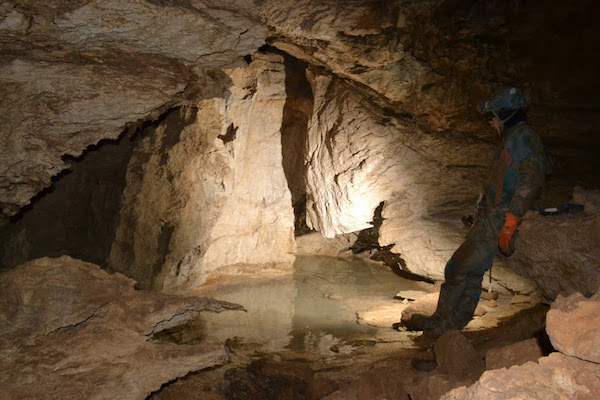
\includegraphics[width=\textwidth]{belowhelm'sdeep.jpg}
\caption{Water chamber below Helms deep}
\label{water chamber below helm's deep}
\end{figure}

A small stream emerged from an obscure fissure which enlarged to an anthropic opening on top. Rhys climbed up into the rift a metre above the water and followed the passage leading off upstream. At every meander, sharp prongs of rock remained, catching on our suits, forcing us to negotiate the climb with care. A few twists and turns followed, until a flat out, damp crawl connected with the base of a large pitch. The rumble of the water rushing down resonated all around, and a slight drizzle dusted Rhys's shoulders with glittering droplets. This was the bottom of the two-waterfall pitch, underneath the pile of  cave sediment that make the floor of Helm's Deep chamber. 

The first piece of the puzzle fell into place. Back at the water chamber, we could see the stream disappearing into a tube. This almost certainly leads to the lower water chamber which is the termination of Sic Semper Tyrannis. In the latter, the water flows underneath boulders to Davy Jone's Locker passage. Swiftly, we caved towards the pushing front, trying to piece together the hydrology of this region of cave. Following the water, past the sump bypass flat out crawl, to the undescended pitch Rhys and Ben had found earlier. At the head, I put in a bolt, backed-up by two sling anchors and tied up a Y-hang knot. When I looked at the remaining length of rope available to descend, I let out a loud curse. Either rope we'd brought was too short on its own after the knots were tied. 

I had learned how tie two ropes together beforehand' whether I'd trust my life with it was another matter. After a few minutes deliberating however, we'd satisfied ourselves that if it had been done to descend 'Godzilla', with not one, or two, but three knots, then surely it could be done again. Not that our own pitch was such a monster, but soon after the take off, the pitch belled out, and after the knot pass, a smooth descent brought me on top of a boulder pile, in a dry chamber. Rhys came down soon after. There was no obvious way on, though the rumble of water could be heard, so we searched for man sized openings between the carefully positioned boulders. Dropping down a few metres brought us to a tight rift, heading west. 10 metres farther, the rift opened onto a small balcony overlooking a sizeable pitch, where the sound from a cascading streamway could be heard. To our left, the spray from the Davy Jones Locker almost reached us, while to the right, the morphology of the pitch suggested a far larger inlet of water down below. 

We were running out of rope and time so we left this last piece of the puzzle for another time. It is probable that the larger inlet is the water from Brezno Slapov, and that the water we followed came down in one of the wet avens of Lethe. Only descending the pitch would prove it, but nonetheless, it was satisfying for us to solve one small mystery of Sysmig.
'
\subsubsection{A new lead in the north}
It was three weeks in the expedition, I'd had a break in Tolmin, and was about to set off for a photo-trip with Rhys to Sic Semper Tyrannis, followed by a visit to the northern reaches of the system and maybe Colarado Sump. The bivi was full of cavers, some actively descending surface shafts nearby, others keen to dig K12. I had a plan to make the washing area somewhat salubrious again. Decades worth of edible matter had piled up over the scree, and penetrated deep underneath the rock cover, slowly turning to an impermeable layer of miasma clogging up the interstices between the cobbles.

It was decided that a good way of draining the water from this area where, after all, mess tins and cutlery were supposed to be cleaned, was to dig a deep trench, removing scree and sediment alike, and to fill the space with fresh scree. I took a shovel, a digger's jerrycan (the lateral face being cut out to resemble a miner's waggon) and a tacklesack. 

Getting the first inches of depth was hard work, filling the tacklesack half-way up, carrying it out of the bivi, and starting again. Very quickly, a foul stench emanated from the hole, hydrogen sulphide from decomposing matter. On the way, I unearthed some old bits of tat and string along with a healthy dose of coal-black slime. After fifteen tacklesacks or so, the hole had a capacity of almost 100L. I stopped then, as the sun beat down on the hole, giving the vapours an even fouler smell. I also had to prepare for the underground trip, but secretly hoped to get back to it later...


'I'm quite excited about visiting the northern bits of the cave' I told Rhys as I put my wet socks on. The camp was silent, even Zimmer could not be heard which meant it was dry on top of the mountain. Oversuit, SRT kit, helmet. A last check and we blew the candles, squeezed the rubber duck and left the shadowy alcove where the tent was pitched.

I descended Big Rock Candy Mountain and followed Rhys to Playboy Junction, through the Leprechaun series, down Memory Lane to Red Cow camp. From then on, it was discovery for me, in the dry sandy passages of No More Potatoes. On the way, Rhys pointed out a rope disappearing up an aven 'strap on the Nitro' he said.Without further ado, we went through a pebbly crawl, up a very long slope, culminating at the start of Smash, a series of breakdown chambers connected by free climbs. Thanks to Rhys's route-finding, we soon broke into Miles Underground, a spacious rift with a boulder floor. This passage was very reminiscent of Wales caving, especially the entrance to Ogof Ffynnon Ddu. 

Soon, Rhys spotted a gap in between boulders from which a small stream emerged. The stream almost immediately dropped into a clean washed chamber. From an alternate route, we made our way down into the water chamber, where a rift in the far wall could be seen to swallow the stream whole. We cautiously had a peek from the top of the drop, and decided it was a promising lead, got busy putting a bolt and tied in a Y-hang. This time I let Rhys descend first. While the higher section of the 15m drop was rigged well away from the water, the bottom third was exposed to the drips, which pooled at the base of the rope. A quick abseil from both of us meant we stayed relatively dry but to our dismay the passage closed down almost immediately. 

I prussicked back up and waited for Rhys, who on his way up scouted for a higher traverse and possible lead. After spotting a likely alcove towards the top, he proceeded to reach it by bridging the rift. When that technique failed, he resorted to swinging, but the rope was dangerously close to the wall so it was abandoned. History might prove us wrong, but from our vantage point, the lead didn't look promising enough to be worth putting another bolt. 

We left it at that and continued our route northward to the very end of dry exploration: at Colarado Sump, which had recently been passed by Jarvist Frost and Connor Roe. Since we ourselves did not carry neoprene suits, we would only look at the duck. Just before the silt banks that announce the end, Rhys took a turn to the right to have a quick look at the Hoover Dam lead, a sizeable aven, not quite vertical, with numerous holds. It was no surprise that Connor had gotten quite high before turning round. At the bottom of the aven through, Rhys spotted a cleft in the wall. A true chattiËre! 

'I bet it's been looked at before' Rhys exclaimed, 'but let's have make sure nonetheless'. Soon we were both on our hands and knees, crawling up. The bowel did not close down immediately, and after ten metres it really looked like a small anastamosing tube, connecting two large passages. Things were looking up, and we switched places so I could lead as well. From the pristine mud we smeared all over the place, it was becoming clear no one had been there before. Thoughts were racing in my head 'What if?'' 'don't die just now?'. After a sharp turn, the passage dropped into an incredibly tight rift. I reckoned that I could fit through the slot without SRT kit and any regard for personal safety. I got wedged up to the hips, before folding. We turned around, and left this thirty metre long tube unsurveyed. 

I was caught short then, as every precaution taken in the morning at X-Ray failed to clear the system for long enough and it became evident that I'd contracted a gut disease whilst digging the trench in the Bivi. Finding a suitably dark corner, I let the tide wash over the rocks. 

Rhys and I then had a look at the duck, going as far as the now well trodden silt banks. We turned around, climbed the smooth bedding plane to Infinity and Beyond junction, whereupon we tried to reach a greater height in the aven. After reaching a suitably exposed vantage point, we decided not to put ourselves in an unnecessarily dangerous situation, and climbed back down. As if to comfort us in this decision, one of my footholds gave way and I slid two metres down the rift, back against a muddy slope. Rhys was well out of the way, but it served to remind us not to trust the rock anywhere. Caves after all are a hostile environment. 

Our spirits were somewhat dampened: there were no impressive finds for our last underground trip of the year and I had the feeling that we had started a decline in cave discovery. Were there any more long horizontal offshoots to be found far below Migovec' We started the long trudge back up to Smash with heavy hearts.

As we were approaching the start of the Smash breakdown, Rhys climbed up on the western side of the boulder slope and cursed as the way on could not be found. Instead, a seemingly insignificant alcove opened underneath a protruding knob of rock. A small pit could be seen beyond. 'Probably doesn't go anywhere right?'. I did not answer straight away, I looked at the beckoning darkness.

Slowly I undid the straps from my tacklesack and left it on the rocks. I jumped into the small  pit, at the bottom of which a tight flat out crawl led off. A few potato sized rocks lay here and there along the plane of bedding, which I shoved across. The crawl carried on downwards for five metres, beyond which I could not see a continuation. The plane disappeared underneath a floor of small pebbles, sloping in the opposite direction. 'There nothing here ' I said, but I didn't wait for a response: as soon as the words came out, they reverberated across the plane, amplified. 'Wait?' I hummed loudly to ascertain that there was a great resonance in the passage. 'There's an echo, there must be something beyond!'.

I crept forward and extended my neck and saw what I had missed: an anthropic opening, and void space beyond. 

'I'm going to dig a few of the pebbles and then go through, take the instruments' I instructed excitedly. 
'Really' Are you sure it's worth it?' came the answer. 

I grabbed pebbles by the handful and dug a way through. Two minutes later I stood on virgin passage in a modest chamber with a rounded vault of solid rock. When Rhys emerged we shook hands on the discovery. At the far end of the chamber, the ceiling came down to meet the white sandy floor. A small opening led to a squeeze I asked Rhys to attempt first. After he went through I followed, with my chest compressed by a nodule of rock in the middle of the constriction. The rest of the body followed, and we stood in a second chamber, very similar in its shape. Going further along, we were faced with a pebbly dig. A small air opening perhaps ten centimetres high was spotted and Rhys insisted we spent a little time digging it out when I voiced my will to turn around. 

He persuaded me to give it a go, so we both started digging the sand and pebbles until the opening was passable. Rhys attempted it first and I followed. The ceiling was still low, and the way on was through tight passage on pristine sandy sedimentary formations where the small drips had collected into ephemeral streams. We crawled on top and emerged into a third chamber of bigger dimensions, a storming lead! 

I wanted to turn around then, to give us a reason to come back the following year. What more than an easy-to-push lead could you want' Rhys came round to my opinion and we surveyed back to Miles Underground Passage. This new lead headed towards the north west, and looked morphologically separate from the main rift leading to Colarado Sump. Where would it go?

\begin{figure}[h]
\centering
\includegraphics[width=18cm, angle=270]{Tolminka at crossing.jpg}
\caption{The crossing of the Tolminka at Planina na Polog, looking towards Kuk--- Tanguy Racine}
\label{tolminkapolog}
\end{figure}

\chapter{2016- Neprehojene Poti} 
\begin{flushright}
\huge \it The road less travelled
\end{flushright}

\section{The rescue}
 \begin{verse}
Arun Paul
\end{verse}

\section{Finding the path: a steep learning curve}
\subsection{The Primadona-Monatip through-trip: impressions}
 \begin{verse}
Miriam
\end{verse}
Izi and Zdenko had both come up the mountain, and as they knew the Primadona/Monatip system better than anyone they offered to take some of us to see parts of the cave we hadn?t gone to. Two teams were formed ? Izi?s ?lazy? team, consisting of Izi, Isha, Sam, Dan, Will F and myself, and Zdenko?s team for those who wanted more of a challenge, who were Zdenko, Rhys and Will S. Zdenko and Co left early in the morning, but we opted for a more relaxed approach and didn?t leave until midday. Our plan was to reach Alcatraz in Monatip, and to spend some time looking around the chamber for the passage previously discovered by Tetley (but never recorded) that would lead to Primadona ? creating a new connection between the two caves.

Morale was high as we set off for the caves, and as it was still early days the abseil to the entrance series was still new and exciting, and not at all soul-destroying. I had gone to the cave only twice before and had never gone deeper than around 200m, so I was excited to see more.

We moved swiftly through the entrance series, descending pitch after pitch until we met Jack and Kenneth near Bear Chamber. They were busy rebolting a pitch head, and unfortunately this meant we had to start using the old rope. This was my first taste of Slovenian style caving, and although I can appreciate the economical approach to bolts and rope, I?m not sure how safe it was. We carried on, and at Risanke (RIP) we passed Zdenko, Rhys and Will S. They had gone to Smer0 and were on their way out. Izi had forgotten to write a call out in the log book, so this was a good opportunity to send a message up to the surface. We soon reached ?Lost and Found?, a junction where the cave passage deviated ? one path lead deeper into Primadona and to Quantum state, but the path we were interested in would take us into Monatip. 

Progress became much slower and we would occasionally have to stop and look for possible ways on as it had been a while since Izi had done the connection and he was struggling to remember certain parts. Our longest stop happened at an aven where the way on turned out to be a hidden free-climb up a waterfall.

After a while, we reached Alcatraz, where we stopped and half-heartedly looked around for a while. Although this had been our purpose in coming, we were all tired from the journey and eager to move on. It was here that we decided to carry on and exit through the Monatip entrance, rather than retrace our steps back through Primadona. 

From that point on the caving became less SRT based and more technically demanding, and although this was more tiring, I was glad for the break. After lots of flat out crawling - during which I was bombarded with flashbacks of the T shaped passage in King?s Pot - and many free climbs later, we eventually reached a very tight squeeze that opened out into a slightly larger chamber. To get through the crack I had to take off my SRT bag for the first time. This made the squeeze slightly easier but no less terrifying. Everyone slowly made their way through, and on the whole it was only mildly traumatic.

After going through a series of unpleasant crawls, we realised that we wouldn?t make it out in time for our call out, so Dan was sent ahead as we hoped he would move quicker on his own.

The rest of the cave was much easier, and although progress was still slow we eventually found the entrance to Monatip, although as it was pitch black outside it took me a while to realise it wasn?t another chamber, and actually the outside world. 

It was an exciting and challenging cave, and overall an amazing experience. 9/10

\subsection{First findings: Quantum State and below}
 \begin{verse}
Miriam
\end{verse}
Terminus
After discovering Quantum State with Rhys and Kenneth and leaving the lead unpushed, a few days later I went back down with Will French. 
Uncertain of how much passage we would find, we brought only a small hand bolting kit with us instead of the heavy drills, and rather than bringing a tackle sack full of rope we planned to pick one up on the way down. 

We went through the abseil and down the entrance series without any problems, although Risanke (RIP) was where we started to lose our way a bit. Will had not gone down this far, so it was up to me to lead the way to Quantum State. We eventually reached the Quantum State entrance pitch, although it hadn?t been a smooth journey ? I often forgot the way on, and during one descent my hair got caught in my descender. It was the first time I?d brought the super friends down into the caves with me, so I could cut the jammed hair off with minimal trauma, but from then on I made sure to keep my hair well away from the rope.

We descended down the Quantum state entrance pitch and quickly reached the PSS survey station marking the edge of discovered passage. After a few short metres we found an intersection, where the passage split into two paths. The more unpleasant looking passage followed a stream, and after pursuing it for a bit as the ceiling got lower and the walls got narrower, we found a sump. Reluctant to survey, we turned back, hoping that the other path would reveal more. 

A short, awkward crawl later and we reached a pitch. Excited that the lead wasn?t dead, we quickly(ish) hand bolted the pitch head ? my first experience of hand bolting. After adding the hanger, we realised that we had left the spanner back at the bivi. Will was keen to go down and said he didn?t mind descending on a single bolt with a semi screwed on hanger, but I had had enough of Slovenian style rigging, so instead we went back up and decided to come back another time.
The next day, armed with a spanner, we completed the bolting, and after some struggling with the rigging (I?d only rigged once before), we descended down, destroying the previously pristine mud floor in the process. 

Almost immediately it was clear that there was no obvious way on, although after some desperate searching, we found a small crack in the wall above a short free climb. Will went through first, and tried in vain to hammer away at the edges, after which I followed through. The chamber on the other side was beautifully untouched, with a small waterfall (a trickle of water) creating a small pool at our feet. There were, again, no obvious leads, but deciding that we had gone through too much effort to turn back, we looked around carefully. After a dodgy free climb to reach the start of the waterfall I found a tight, dank passage following the stream. This, however, led to yet another sump, so we called it a day and started to survey back. 
Surveying proved to be especially unpleasant, as we were knee deep in water when surveying the sumps, but as we hadn?t discovered much passage, it thankfully ended soon.


\section{When dreams come true - Leads under Rokovo Brezno} 
\subsection{The discovery of Karstaway}
 \begin{verse}
Tanguy Racine
\end{verse}

I was keen to go caving with Jack, not having the opportunity to do it in 2015. We'd put quite a bit of work into rigging the abseil to Primadona, and things were looking up in the Galerija branch of the cave. Memory of previous leads in this zone had not faded as much as for the rest of the cave, and after the first spark of exploration in Quantum State it was time I got some findings under the belt.

On the surface, we had a good plan: going in Galerija, and traversing at the top of Quantum state, we'd be able to reach a zone with several open leads (as shown by the 2011 survey). We only had one pitch to rerig on the way: the 20m hang dropping at the start of Smer0 and Galerija, which had been dubbed Knot So Great. There was an early start in the Bivi and early enough we reached said pitch. Bolts in, rope tied, descender rigged, I descended, placed a rebelay and frowned upon the rope rub that had appeared just on top of it. The old slov rope was within reach, tied to a rebelay two metres above mine. I grabbed the rope, cut it and tied a deviation. The bundle of rope dropped to the bottom. This done I went down, quickly finding myself under a small drip. 

The bottom of the pitch was a larger space, draughty and noisy, littered with sharp, shiny white boulders of all kinds of sizes. At the bottom, we were joined with Rhys and Will Scott who'd caught up with us and had a plan to push the stream underneath the same boulders. Jack and I pressed on in the windy Galerija, glancing at the floor and ceiling, looking for leads others might have missed. There was a tight, loose cobbly tube before Quantum State I popped my head into but thought better of it. Past Quantum state, gingerly, ever so gingerly Jack and I traversed over the pitch head, sending a few cobbles and blocks of mud down the black throat of the pitch. On the far side, new territory awaited: a rift, guided by a fault plane, with thick protrusions of white rock and a howling draught.

After a few twists, the floor dropped two metres, into a puddle of brown mud. We dropped that as Jack muttered ?Should be fun to climb back up'. There were a few tens of metres of meandering rift with a high way along the top of the rift, leading to committing crawl over boulders. We'd lost the draught there so opted for the lower way down, hugging the bottom of the rift, and following the gale. A few more drops, and around a corner a large yellow tacklesack. Beyond that, a rope led into the darkness of large pitch.

After a cursory inspection of the hangers and rope we decided it was okay to descend. The drop was a clean hang, perhaps 30m deep, in a pitch some ten metres in diameter. At the bottom a cairn had been built well out in the centre. Jack had been quickly scouting the ways onwards. It seemed we'd reached TTT, as this was what Zdenko thought likely. If it was, then the connection had not been marked on the survey. The way down was obvious but tricky. The first free-climb down was not very tricky, nor the second. The passage turned left, there was another down climb where the passage wall widened underneath the ledge we'd come to. There were plenty footholds, but I remarked ?Those free-climbs are looking more and more dubious'. 

Jack took over the lead for the next drop, which was frankly terrifying: traversing around a ledge, hands on the opposite wall till the walls got far enough together that we could bridge down. At the bottom we considered what we just did, with doubts gnawing at us: surely this should have been rigged? Upon inspection, the way on didn't bear any footprints, nor any other sign of previous discovery. We were then almost certain what we found next was virgin passage and the way on looked promising: wide, with a small stream and a howling draught.

At the bottom of the down climb was as good a spot as any to have a lunch break, and the cheese and fish we'd brought down made for a very welcome fare. Without delay Jack led the way into the streamway. For two metres it was storming. After that, it degenerated into a tight rift, with a large, pointy boulder providing the chief obstacle to easy progress. The passage went on nonetheless, and what's more the loud splashing of a waterfall could be heard further on. After a short way, the width of the passage increased, and we saw the water, went past it to reach a ten metre aven chamber where the direction of the passage veered into the west. A small series of scalloped passages led to a white dry twisting rift. The water plunged somewhere underneath, but we preferred the wider, upper level dry passage, which continued to a pitch head. The rift itself was very white, with a white clay to silt draping the knocks and crannies of the walls. Within this matrix there were larger granules of haematite, no bigger than a couple millimetres. 

We contemplated the pitch we'd just found: truly a remarkable find because of the strong draught and the possibilities of deep shaft bolting that opened up. We only needed a suitable name for our discovery. Blessed karst? Jack laughed but wasn't convinced. ?The leads here were abandoned, so... how about ??Karstaway''?'. And the name stuck. We decided to turn around, conscious that we still had a fair bit of surveying to complete before racing to the surface to announce the good news. 

Not having spotted any of the PSS's indicating the previous pushing front we opted for a full resurvey to the head of Quantum State pitch, which Rhys had marked the day before. We obviously got slightly chilled doing the surveying in the tight draughty rift, but at least we had good line of sight, and made up for the cold by being speedy. At our lunch spot it was possible to look upstream, and this route died conclusively in the matter of seconds: a 15m aven, with haematite pebbles and a calcited sediment formations (chiefly fossilised water droplet imprints on the white clay). Climbing back up the scary freeclimbs convinced us they needed to be rigged on the next venture. 

At the top of the 30m pitch, we started hearing voices. Will and Rhys were coming our way. We joined up exactly at a tricky climb, a flat mud floor at the bottom, and a lip of rock to hang on to 2m above the floor. Little in the way of holds, doable but rather annoying. Now I'm not a civil engineer, but I thought that raised platform was a sensible option. In a fit of near madness I started rolling large boulders on the floor, piling them up to form a large cairn. Gingerly, ever so gingerly I leapt on it and grabbed the walls of the rift, pulled myself up. I got out of the way, and Jack did the same. Our laughter was interrupted by the dull thump the edifice collapsing on the mud. 

Soon after we finished our survey at the head of Quantum State. It was not too late yet to be out by sunset, and following Rhys's lead we made a steady way out. The dream of another pitch series was on...

\section{Exporing the Limestone Pavement} 
 \begin{verse}
Tanguy Racine
\end{verse}
What I?ve taken to call the Limestone Pavement is a region that has not received the attention it deserved during the past few years. This ?flat bottomed? feature is truly remarkable, covering an ellipse of semi-axes 100m and 200m, oriented NW-SE, lying between the Bivi and the peak of Migovec. The dip of the beds in this area is towards the south -west, therefore exposing bedding as steps between 1.5 to 2m. Two perpendicular arrays of linear joints are exposed and enlarged by meteoric water solution. Elongate pits choked with snow and ice abound in the area, making cave prospection difficult. This area is the true southern part of the plateau, hosting the 110m deep pot of PF10.  At depth, this is where the ramifications and active streamways of the Atlantis branch were found. Could this region provide entry from above into the southern extensions?

I had managed to reconnoitre the area in 2014, following Jarvist?s advice that little else than PF10 had been discovered. On my own, I packed a small bag with GPS, gloves, light and oversuit to check out as many likely holes as possible. This was a foggy day and I logged 8 caves or beginnings thereof that I had visited. Some died conclusively as the wall rock closed down on the passage, some I hadn?t got rope to descent, others choked with ice and scree. One I got slightly stuck in, for want of digging enough scree out of small squeeze. As I advanced the rotation of the cobbles denied the possibility to back out. The only way was forward, into a small aven chamber which died immediately. Shimmying forward got me unstuck but the ordeal highlighted how unwise it was to go too far on one?s own. When I got out, the fog was thick, the breeze cool, and unbidden thoughts about one?s vulnerability up in the mountains sprung to my mind. I carried on with my search more cautiously. In the end, there was one cave I?d spotted (several entrances, including an aven) that had grabbed my attention. Unfortunately I lacked the rope to descend it on the day, and for another two years it waited.

As it happened, Will, Arun, Kenneth and I planned to go back down to Tolmin mid-expedition. The day before going down there seemed to be a lot of agitation in the bivi. Recent finds of large chambers, horizontal passages and shaft series had gripped the imagination of the group. Little few cavers remained on the surface on the day, but among those Will Scott helped Janet, Dave and I cleaning and clearing the Bivi (not in that order). With the sunshine, an afternoon ramble across the plateau with a light caving bag seemed reasonable. With the morning chores completed and plans for the day finalised Janet Will and I set off, trodding the ?old Mig path? Janet had been trimming and clearing up after several years. From the Bivi it led along the top of the M16 escarpment, gently curving to the SE. Gardener?s World Valley and Area S unfolded in front of us, then in the distance we spotted the Razor hut, and further still a line of limestone crested mountains heading south, till they disappeared in the haze. This panorama was a feast of soft greens, greys and blues. At the end of the clear path, we turned due south towards the peak of Migovec, going across a grassy, hilly terrain, circumnavigating the shakeholes. On our right, we passed the Amphitheatre, a large 50m wide depression with excellent acoustics. On the verge of the Limestone Pavement, the ground dropped steeply forcing up to pick a snaking path towards the head of the valley, past some of the rare trees of the Plateau that do not appear to suffer from dwarfism. 

The Pavement was as I remembered, bare limestone beds, deep shady cold pits exhaling their cold breath. We kept to the northern, deeper end of the valley, choosing a careful path amidst the boulders. With the GPS we found the cave of interest quickly, had a look and pressed on ?downstream? - the pavement is a hanging valley, completely dry. This led to M24, a depression of the same scale as the Amphitheatre, open to the north, boasting a 20x20m snowplug. At the far deep end of the shake hole, a small rift could be entered, a rift that dies within five metres, choked with boulders. On the eastern cliff face  (I am using this word here because of the asymmetrical nature of the depression), a large entrance to a cavity could be seen. It is certainly possible to climb into it and drop a rope for safety, but it is unclear whether this would only take one up into a small shaft that once led into a cavern. 

Past M24, we found the ?old mig path? again, in much better state than a completely abandoned trail would be. Cuts on the trees were old, maybe two or three years, but no more. I understand that it was once the highway from Kal to the Plateau, creeping up the eastern rather than the western slopes of the mountain. It must cross the Mig southern cliff face. Some 200 to 300 metres of decaying limestone, and underneath a high angle scree slope, funnelled into a couple of dry valleys. All the way to Ravne. 

Indeed the path led to the start of a vertigo-inducing traverse of face of Migovec, but before that it took us to a gorgeous panoramic from the high eastern promontory. All that we had seen before and more unfolded before our eyes, from Skrbina to Zabiski Kuk, thence down to Tolmin and up to Grusnica. And everything beyond, Most-na-Soci, the plain of Trieste. Most of all, the entire bowl of the Razor alp, the southern apron of Migovec where Coincidence cave lies, all of it crystal clear. A crow?s nest. We turned around after a few minutes of silent contemplation and climbed back up to TR01, the cave in waiting. 

It took only a few minutes for Will to learn how to hand bolt. I demonstrated first placing the back up bolt while he looked on. Janet sat on the pavement and shared the little treat she had brought along: crackers, jam, mountain cheese. Will put his kit on and got to work with a gentle tap tap tap tap  of the driver into the hard limestone. He acquitted himself very well and before long the only other bolt placement needed to complete the trivial descent of a 5 metre drop was done. Without effort he rigged the pitch and descended. I commanded him to remain silent, but a few ?ohs? and ?ahs? came back up. I followed quickly dropping into a small chamber.
?It might not die immediately? Will said, thereby attracting the anger of the cave deity. Though not all doors were closed, none went very far. 

The cave was by all accounts a small one. It sported a modest chamber, linked to an aven (5m) to the west, choked with ice and rubble. Right by the landing there was a draughting snowhole. At the far end of the chamber, a small tube, littered in wet, sharp pebbles led off for  a few metres in another chamber, of even smaller dimensions. The walls were covered in glittering ice, with a few curtains and stalactites (of ice) shining to our lights. I took a few photos, and proceeded to descend the snow hole. Will looked at me with a solemn face. Here goes another nutter he might have thought. We were in T-shirts, and the temperature within the cave, in the draught was not balmy. But wait, wasn?t it obvious? A snow hole, the draught, what massive chambers could lie beyond? I did not hesitate and descended.

Unfortunately the rope was at an angle to the tube of glistening wet snow, and started rubbing, then sawing, then hacking big chunks of snow down on me. Quickly I abseiled till my feet touched the floor. I put my weight on them and the floor went from under me, a pile of rubble flying out. I caught the rope, and pivoted to see what gigantic chamber I?d landed in. 

It was cosy, a 2metre wide rift, degenerating to next to nothing at all downwind, but it was worth it, for a glittering, metre long, thick carrot like stalactite hung from the righthand wall. It even had growth rings, refracting the light in all directions. I urged Will to come down. He absolutely had to see it. And he did, though he cursed me a little for the ice shower. I was not going to let him off for this, so I asked him to carry my flashgun in the most cramped positions imaginable, in the snow tubes that led off. The resulting play on light and shadow in the mini-wonderland was worth the effort.

Back in the sunshine, we derigged the cave, ate the remaining crackers with Janet, and set off in search for PF10. Once the boulder-filled shakehole was located we carried on uphill towards the bivi and found the grassy N-S avenue which leads to camping site. Within minutes we were back in the fading sunlight at the top of the Plateau and headed to the Bivi where the dinner preparation awaited. Will and I also baked some cocoa and ground almond flapjacks, which earned the nickname ?Tanguy Treats?. We were low on underground food, and this glorious enterprise averted a chocolate bar crisis. Donuts were deep fried and given to the earliest returning cavers. Jack and Kenneth, then Rhys and Arun and finally William and Miriam. Again there were tales of more horizontal passage and a typical late Bivi night.


\section{A foray into the original pitch series} 
 \begin{verse}
Tanguy Racine
\end{verse}


I?d never gone expedition caving with Clare. We had managed to cross paths at X-Ray or on the surface in 2014 and 2015 so we decided to make up for this. We planned to cave after a mid-expedition break in Tolmin spent walking around to the Tolminka gorges and then to the Izvir Tolminke where Will Scott and I got thoroughly drenched. It seemed like exploration in the new shaft series was dying down slightly after the horrors at the bottom of Upside Down chamber so we decided to have a look at the original, older, deeper shaft series, past the infamous Brezno TTT (infamous because it looked wider than most shafts in the system with the exception of Silos and Happy Monday).

It had also not been visited at all during the summer, despite its proximity to the entrance and the relative route-finding ease, but with very good reason until now: we wanted to find our own way down. When had it been last visited? There was also another interesting nexus en route to TTT: Mandare. This crossroads was marked as an open lead on the 2000 survey, and the drawing of it remained unchanged in the 2011 survey, though additions to the deeper series had been made. Why was it so? Finally, we thought it would be good to gain knowledge of the upper part of the original deep series as its passage morphology might give off clues as to where connections between the two shaft series are likely to be found, and whether it had any potential for mid-depth horizontal development as seen in Karstaway. 

From Sejna Soba, the whole of the way to TTT was a basic rift. There were obstacles, of course, how not in a cave of generally small dimensions, fault controlled and full of choss? The odd climb up or down a waterfall, the emergence into the bottom of an aven. And there were leads. Closest to Sejna Soba was a little carbide arrow pointing the way at a junction, but taking the other option took us to the take-off of a 10 metre deep pitch. This junction is noted on the 2011 survey as an open lead, and admittedly, the pitch is found directly on top of another horizontal branch of the cave. Could it provide another, easier connection? Further on it the impressive Povezava Aven, a 20x20m aven, boulder strewn. It is slighlty slanted however, with the eastern wall dipping towards the west. 10 metres from the floor, a dark recess, 5 metre wide  that could be a window into horizontal passage was spotted. The bolt-climb appears to be a straightforward one, and still very close to the surface. Importantly, Povezava is amongst the easternmost points of Primadona sensu-stricto, and going further east might yield a pathway into much barren mountain so far.

TTT was impressive. If one could find the way to access the pitch from the very top, it would be a good 80m deep, and 20-25m broad throughout. The passage joins in about halfway down the pitch. But where was Mandare? Supposedly the connection between Stara Jama (the old cave) and the Povezava branch, we saw no sign of a passage joining in at right angles to our rift. Though we spotted an aven it was nothing like the drawing on the survey. In all probability, the Povezava branch joins in at the bottom of a pitch, once accessed from the top through Stara Jama. The old way could have been derigged later on. No one had visited the Stara Jama branch, focussed as we were on the new shaft series. 

After rerigging some of the scaries hangs of TTT (a smaller parallel shaft joined in towards the bottom of the pitch, the wall between the two I assume gradually thinned down to a few feet where the last, loose and rusty hanging rebelay was), we bottomed this might pitch and searched for the way on. On the far, southwestern corner of the almond shaped shaft  we eventually found a small draughting rift leading off. Had we missed an obvious way on? We spotted a small drop that had been rigged, descended and reached another climb down. Seeing no ropes, I was hopeful that this was maybe a small side passage no one went back to, but it clearly went on and the draft was strong. The drop led to an obvious junction of two rifts.

Clare spotted what she described as a landing cairn, and after placing a beautiful ?Y?-hang, it became clear that someone had been down. There were abundant footprints on the black-and-brown mottled floor. Further along the rift, downwind past several traverses where drops underneath the false floor got deeper and deeper we reached the ropes. There were many of them, some muddy and attached to homemade hangers, others cleaner with shiny krabs and through-bolts. A set of ropes protected a traverse across a pitch, the other went down.

Since we had not explored the upwind passage at the junction, I proposed that we enter a few metres in the book. Clare agreed so we walked on the mottled floor up into a textbook example of a phreatic tube later turned into a vadose rift. It meandered in a lovely manner, but not for long, soon we were crawling in between mammoth boulders. To our right, there was a small aven which we thought we recognised from before. It seemed we had returned underneath the Brezno TTT rift. As we continued past it underneath another enormous boulder we heard the echo, and drips of a larger chamber beyond, TTT itself not doubt.

Only it was not. It was something else, a drippy, boulder strewn chamber that looked curiously similar to TTT. The water came from a little pitch higher up and the chamber itself had the shape of a kidney. Turning left, the ground rose, and the chamber was dry. Keeping to the left hand wall - we had done an 180° turn at that point, the draught changed from upwind to downwind, and the floor sloped down to a pitch head. Twenty metres deep maybe more. It probably reconnects with the original pitch series, it must, with all the snaking around we can?t have moved off that far. We having rope, drill power and metal work did not bolt down this new pitch. We placed our bets on the already rigged way down Ajdovscina pitch. 

So after a short survey we came back to the bolted pitch head. The traverse was almost an obvious choice, the precedents in Migovec abound: stay high, avoid the water for inevitably disappears down impenetrable cracks, and take your share of glory. The bolts were sound, and the rigging adequate but halfway through I did question my sanity. 20 to 30 metres below, the continuing pitch series awaited. On the far side of the traverse a short 5 metre stoop led to a further pitch head, dry this time. The rope was still dry and mostly clean, the ?Y?-hang as inviting as any. Clipping into the traverse line I swung over drop, 20m at most and could see that it was a clean hang, landing on a rubble floor. There was still a heap of unused rope there. 

We whizzed down and explored the bottom of the dry pitch. A sloping mud and rubble floor, with the skeleton of a bat, no dry horizontal way on and around a corner, a large window looking into the previous pitch. We decided to use the excess rope to rig down from the window and back into the main way, bypassing the scary bolts. Another beautiful, wide ?Y?-hang later and I dropped another 10m to reach a ledge, protruding from three sides of a pitch. On the far ledge, a traverse line brought the Slovenians? way down away from the spray and the unstable boulders. With the water on our side of the ledge we opted to mimic the previous way down. 

Three or four more bolts later I prepared to go down the next drop. The lights couldn?t reach the bottom, but I could see the ropes in place running from one wall to the other like a loose, lonely spider web. Again mimicking the existing rigging I placed two rebelays, and reached a large bouldery ledge. There again there was a profusion of ropes: a rope leading in through the boulders high-up from the last rebelay. On the right hand side of the ledge there were two ropes descending the next section of the pitch. A blue rope which could be accessed by traversing on the broad ledge to the first anchor. And a white rope, a ?Y?-hang bolted from a rift on the far side of the pitch. Could the rope leading into the boulders find its way to this far rift?  How else to reach it?

When Clare joined up with me, we had a little break and considered our options: we had were precious little bolts left, next to no rope. We didn?t chance using the in-situ rope, instead turned around, with the aim to sort out some of the rigging on the way out. Though we had not found where Jack and Kenneth?s route joined up with the old pitch series, we?d gained the knowledge of the route, its obstacles and gauged the state of the rigging in this forgotten bit of cave. 

Interestingly, we didn?t see any obvious pitch coming in from Déjà Vu as we went down, and looking at the survey, it looks like there is a sizeable distance between Ajdovscina and the pitch head, perhaps as much as 40m horizontally. Can this be the next way down deep?

The survey of a sewer - Cloaca Maxima

The plan was simple: Maffi and I were going to go in Primadona, pick up some rope at Sejna Soba, go in Monatip, then towards the NCB connection and drop a pitch there. Maffi knew the way to the connection given he?d participated in the effort to push Monatip during the preceding year.  I foolishly assumed he also knew all about Primadona to Monatip, this is was grave mistake. Still we agreed to meet at the entrance of Primadona the following morning. 

?What time?? Maffi asked. Now careful, you must not be seen to offer an easy option, you?re a hard caver.

?As early as you wish? I answered. This was not the expected answer, I could see it on Maffi?s face. But then I never really lie in bed.
`
?Maybe ten then?? I offered, as it had become almost a habit to go caving early, in order to come back up for dinner. This time round, dinner in the bivi after the day?s push was not on the cards: it was going to be a long, arduous trip, with glorious, remote exploration involved at some point. Maffi would be coming up from Kal, picking a path through the boulder slope. I would abseil from the top, with the drill, battery and metal work. I couldn?t wait for the trip to begin and the wine did nothing to quench my enthusiasm. Au contraire?

The next morning was quite still, with little wind among the dwarf pine bushes. I found a deserted bivi, all cold grey rock and ash, with pieces of ?comf? scattered amongst the remnants of the previous night fire. Even the soothing sound of tarps billowing in the breeze lacked. I rustled up a quick breakfast of biscuits and cheese, cold vitaminski and took it out of the shakehole, to sit on the promontory overlooking M10. 

Then followed the usual shuttle between the tent and the bivi, gathering all the essentials for the coming trip: food, water, gear. Finally it was time to stride across the plateau, to the start of the abseil. 

The silence of the morning was broken by the movement of pebbles underfoot, and soon I clipped into the last drop before the entrance, where Maffi was waiting. I zipped down the rope and we greeted each other, upon which Maffi started to change into his caving gear. As he sat on the grassy ledge, he laid his kit all around him and proceeded to kit up. He had the unfortunate notion of leaning back when putting his socks on: this pushed one of his hiking boots over the edge. I could only look on, clipped to the rope as the shoe rolled down the boulder slope. Even when it was out of sight, the crash of boot on rock could be heard at repeated intervals. 

?Nooooooo! Why does it have to be me?? he cried in anguish. 

As far as I knew, the boot might have found its way down to the Tolminka. Still, I offered to climb down to have a look for it, over the first 150 metres of scree that led to the Kuk path. As it happened, the missing item had not gone far and Maffi found it himself, but I had time to climb down to the path and up again before realising that. We spent a surprisingly long time trying to figure out what each other meant: 

?Tanguy? (inintellingible) ?  up? ?

What?? 

?? found it ?? 

?No I haven?t found it! Have you found it?? 

 ?? No ? up?  
 
?What?? 

?? see it ?. up ? back? 

?Okay I?m going back, Maffi have you found it? I can?t see it?  I couldn?t see the shoe at all, and my wanderings had led me far from the usual access path

?No ? Come back ? I have it?

?Okay?

I traversed across the scree to get back to the less insane route, climbed up, traversed underneath a little bush of dwarf pine, grabbing the thick, flexible branches as holds, climbed up a little bit more and stopped at a wall of dwarf pine, crowning a small ridge of rock. I hadn?t climbed down this way, but I wasn?t going to let vegetation defeat me. The going got tricky as the slope was steeper than anticipated, and soon I would only be pulling myself up the branches, with little or no footholds. Clambering back down the lip of rock was out of the question, so I had to traverse to the right  hand side, back to the scree slope. I breathed a sigh of relief when I reached the fringe of the pine bush, and carried on up, back to the entrance. 

I was relieved to see that Maffi had found his shoe and after all these tribulations, we were ready to go underground. I pointed out the different branches as we passed them, at Lost and Found junction, at the corkscrew climb, and finally at Sejna Soba. Maffi was quite surprised that, at the time, there were no signs indicating the ways out, or on, or about the cave. Indeed, we?d applied our PSS and paper notes policy to the newly discovered passages and omitted to do the same on the trade routes, relying on our own experience of the cave. This was exactly what had led to memory of the leads, and ways in Primadona to fade in the first place. On a later trip with Tetley, and on his urging a few notes were left at the key nodes of the cave.

At Sejna Soba Maffi picked up his bag of rope and a small amount of metalwork he?d placed there the previous day on his reconnaissance trip into Primadona. Had I heard that right? It transpired neither of us knew the way to Monatip, other than it was ?up this rope? hanging in the main chamber. How difficult could it be? Monatip was a simple cave, with little in the way of route finding, save at the beginning where the passages leading to NCB had been found.

I ascended first, reaching a very exposed traverse over the chamber into a small rift. There was a carbide arrow leading up to it, and I almost climbed it but Maffi appeared at the pitch head, reading a note in Slovene which said? traverse more?. The very exposed traverse turned into a madly exposed traverse, leading to yet another small rift, whose only redeeming feature was an exquisite calcified gastropod fossil, weathering out of the rock. The rest was carnage, a tight, sharp draughty rift we had to climb up in, till we broke out into a large aven. There were a few footprints around. The rift continued on the other side of the aven, this led to another chamber, with a possible climb up on the far side. 

The main problem with Monatip was that we expected the way to be hard, mad, dangerous even. This meant we had to try every way up before ascertaining that it really wasn?t ?the way on?. The climb up was largely vertical, with few footholds and could in no way be attempted without utter disregard for one?s life, so we turned around and explored a few more likely holes, with an entertaining loop I can?t begin to describe. We concluded the way must be somewhere else, so we doubled back down the sinuous tight rift, back to the traverse of death, and traversed more.

As if by magic, the going became easier, and soon we spotted a rope going up an aven. This was it, now we couldn?t get lost! At the top of the pitch, we spotted another rope, and our spirits rose a little. We celebrated victory too quickly though, as the pitch head was a boulder choke, with a possible way down into a boulder strewn  chamber, which we explored. The far side was climbable, but this led through to more wedged boulders that had not seen much passage. With a bit of looking around back the pitch head, I spotted the cairned way on, and we carried on our way up. The boulder choke gave way to a phreatic tube passage, and there was even a Slov PSS by a small round chamber. The going was not particularly easy, but we had the draught and the way was well trodden. The passage levelled out and grew bigger, with the signs of an obvious ancient rift streamway going down. Prod marks on the soft mud of the ledges indicated that the way on was up into the rift, and this gained the continuation of the phreatic tube. There, the sediment was churned and flattened by the passage of cavers till we reached a clean-washed aven. With no marks of wellies to indicate the obvious way on, we spent half an hour trying each and hole within this space. We found another oxbow loop, looked everywhere underneath the boulder floor of the aven, but still could not find the way. 

After having a rest, some chocolate and thinking about our predicament, it became evident that we would not complete the through trip from this end of the cave, so we decided to turn back and enter via Monatip to find the way. If we could not push today, at least we would gain valuable knowledge about the cave. 

Somewhat disappointed, we turned around, going down the phreatic tube back to the start of the boulder choke. I started following the cairns but Maffi spotted another neat stack of stones leading away from the pitch head. Curious to see where it led, we soon broke out into a massive aven, which I interpreted to be Alkatraz. This was an opportunity to try out the new route Jack had pioneered early on during the expedition. I found a scramble up boulders on the right hand wall, into a small chamber, and on the opposite side, a little slot through the boulders that was the way down the the Spiral Climb down. 

I reported this back to Maffi, and we opted for the easy way out. Very soon we started motoring up the entrance series of Primadona, and in no time at all, we climbed the snow slope to enjoy the afternoon air on the grassy ledge. We sat there for an hour or so, sharing caving stories and tucking into a nutty fruit mix of Maffi?s own concoction. For a while I tried to guess what was in it - it was after all very fine grained - I got the fig and pistachios after a while, but missed the peanut, the linen and sunflower seeds. By all accounts it was delicious, far surpassing the good old raisins and peanuts. 

We put our gear on again, leaving ropes, metal work and survey kits by the entrance of Monatip to travel ?light?. The cave begins with a pebbly crawl, upwards into the mountain side, branching, before the first pitch. The next section is very straight, with an alternation of abseils, climbs and traverses before reaching the big chamber. Twenty minutes in, we were still only 6 metres below the entrance. The chamber itself is a big aven, with a thin 9mm rope leading up to the connection passages. Maffi led the way up to show me the beginnings of the ?connection galleries?. The SRT was innovative, with a pitch bypass that allows one to clip in at the highest rebelay, only a few metres before the top. Most of the rocks were loose, and the holds on them were tenuous at best. Still, I was soon shown the start of a long crawl. We turned round there, and descended back to the Big Chamber, where the other way on was the original Monatip rift that had been connected to Primadona at Sejna Soba. 

We scrambled down some huge boulders and entered a small muddy rift. Very early on there was a squeeze which we passed easily, then a window looking into a pitch maybe 20metres deep, then another squeeze best attempted feet first, as it pops out over a drop. At this point, the rift widened, with two broad ledges on either side. Maffi bridged forward a little, and a couple of metres underneath we spotted the ropes going down. Reaching them was going to prove problematic. 

The walls were slick, the good sound holds few and far apart, and we decided that we?d used up all our free climbing enthusiasm for the day. Upon turning around, we spied another passage that merged into the rift, right next to the one we?d come from. Thinking that it could provide us with a safe and sensible way down to the ropes we climbed into it. 
A small upclimb broke through to a small rabbit warren of a chamber, with many phreatic tubes leading off - most being too small to follow. It was a worthy find, but the best was still to come. The obvious way on was the largest phreatic tube, plastered with mud on the floor, with a little film of water on top. We followed the footprints until they stopped. The tube went on.

?It isn?t obvious anyone?s been here? I remarked. Further on, the evidence was unequivocal: pristine mud that anyone crawling past would have sunk their knees into. There was a moderate draught, and although we lacked the survey instruments to survey whatever this passage led to, the thought of discovery spurred us on. The tube carried on at a shallow angle for some time, before breaking in a chamber where some of the ceiling had collapsed inward, and then been covered with the same mud as most of the passage. 

At the far end, going down was the continuation of the tube but Maffi managed to climb up into the ceiling rift for little distance, deciding that it did go on past where he stopped. I scouted the boulders at the bottom of the chamber, finding another smaller crawl on mud clasts that doubled back underneath the way we?d just come down. I went in as far as five metres, the passage however continued for another visible ten.

The obvious way on hit a major joint plane perpendicular to the passage, but the tube had found an aesthetic way of bypassing it, by a 3m climb and 2m descent right afterwards before resuming its rough SSW course, contained in a single plane of weakness. The water had disappeared, and the walls became cleaner with a black cauliflower calcite cover. This was very similar to some of the ornaments seen in the entrance series of Primadona slightly further up from the Corkscrew climb, or indeed lower down still in the tight rift of Karstaway.
We spotted a junction, with an upwind passage joining the main way on the right at a high angle, followed by another, where the passage came in perpendicularly from the left handside. At this point, the passage widened slightly, and rift appeared in the floor, and ten metres further on we broke into a large, high aven a couple of metres off the floor. Giddy with excitement I climbed onto the clean, white boulder floor and shone my light around. 

The ceiling of the shaft was lost into the distance, between 30 and 40 metres above, and the aven itself had an oblong cross section, ten metres wide, twenty across. We?d come in from the eastern wall, and at the floor level on the opposite side, the small crawl resumed. I popped my head in and content to have found the draught again, and a probable continuation. How long could this simple hands and knees crawl and stoop carry on for? By our reckoning we?d branched off the main Monatip rift towards the west, towards Primadona. We could not possibly go on forever in this direction, but without the survey it was futile to gauge how far we?d come.  I was ecstatic that we now had several small leads quite near the entrance of Monatip: the junctions, the continuing crawl and the far southern side of the shaft where a climb between the walls revealed that there was a twin aven waiting to be descended. I had also a very clear plan for the following day: survey those hundreds of metres of passage, and continue the exploration. It was almost a guaranteed win, and I would have no trouble recruiting a keen person to see our newly discovered ?nice gallery?.








\begin{figure}[h]
\centering
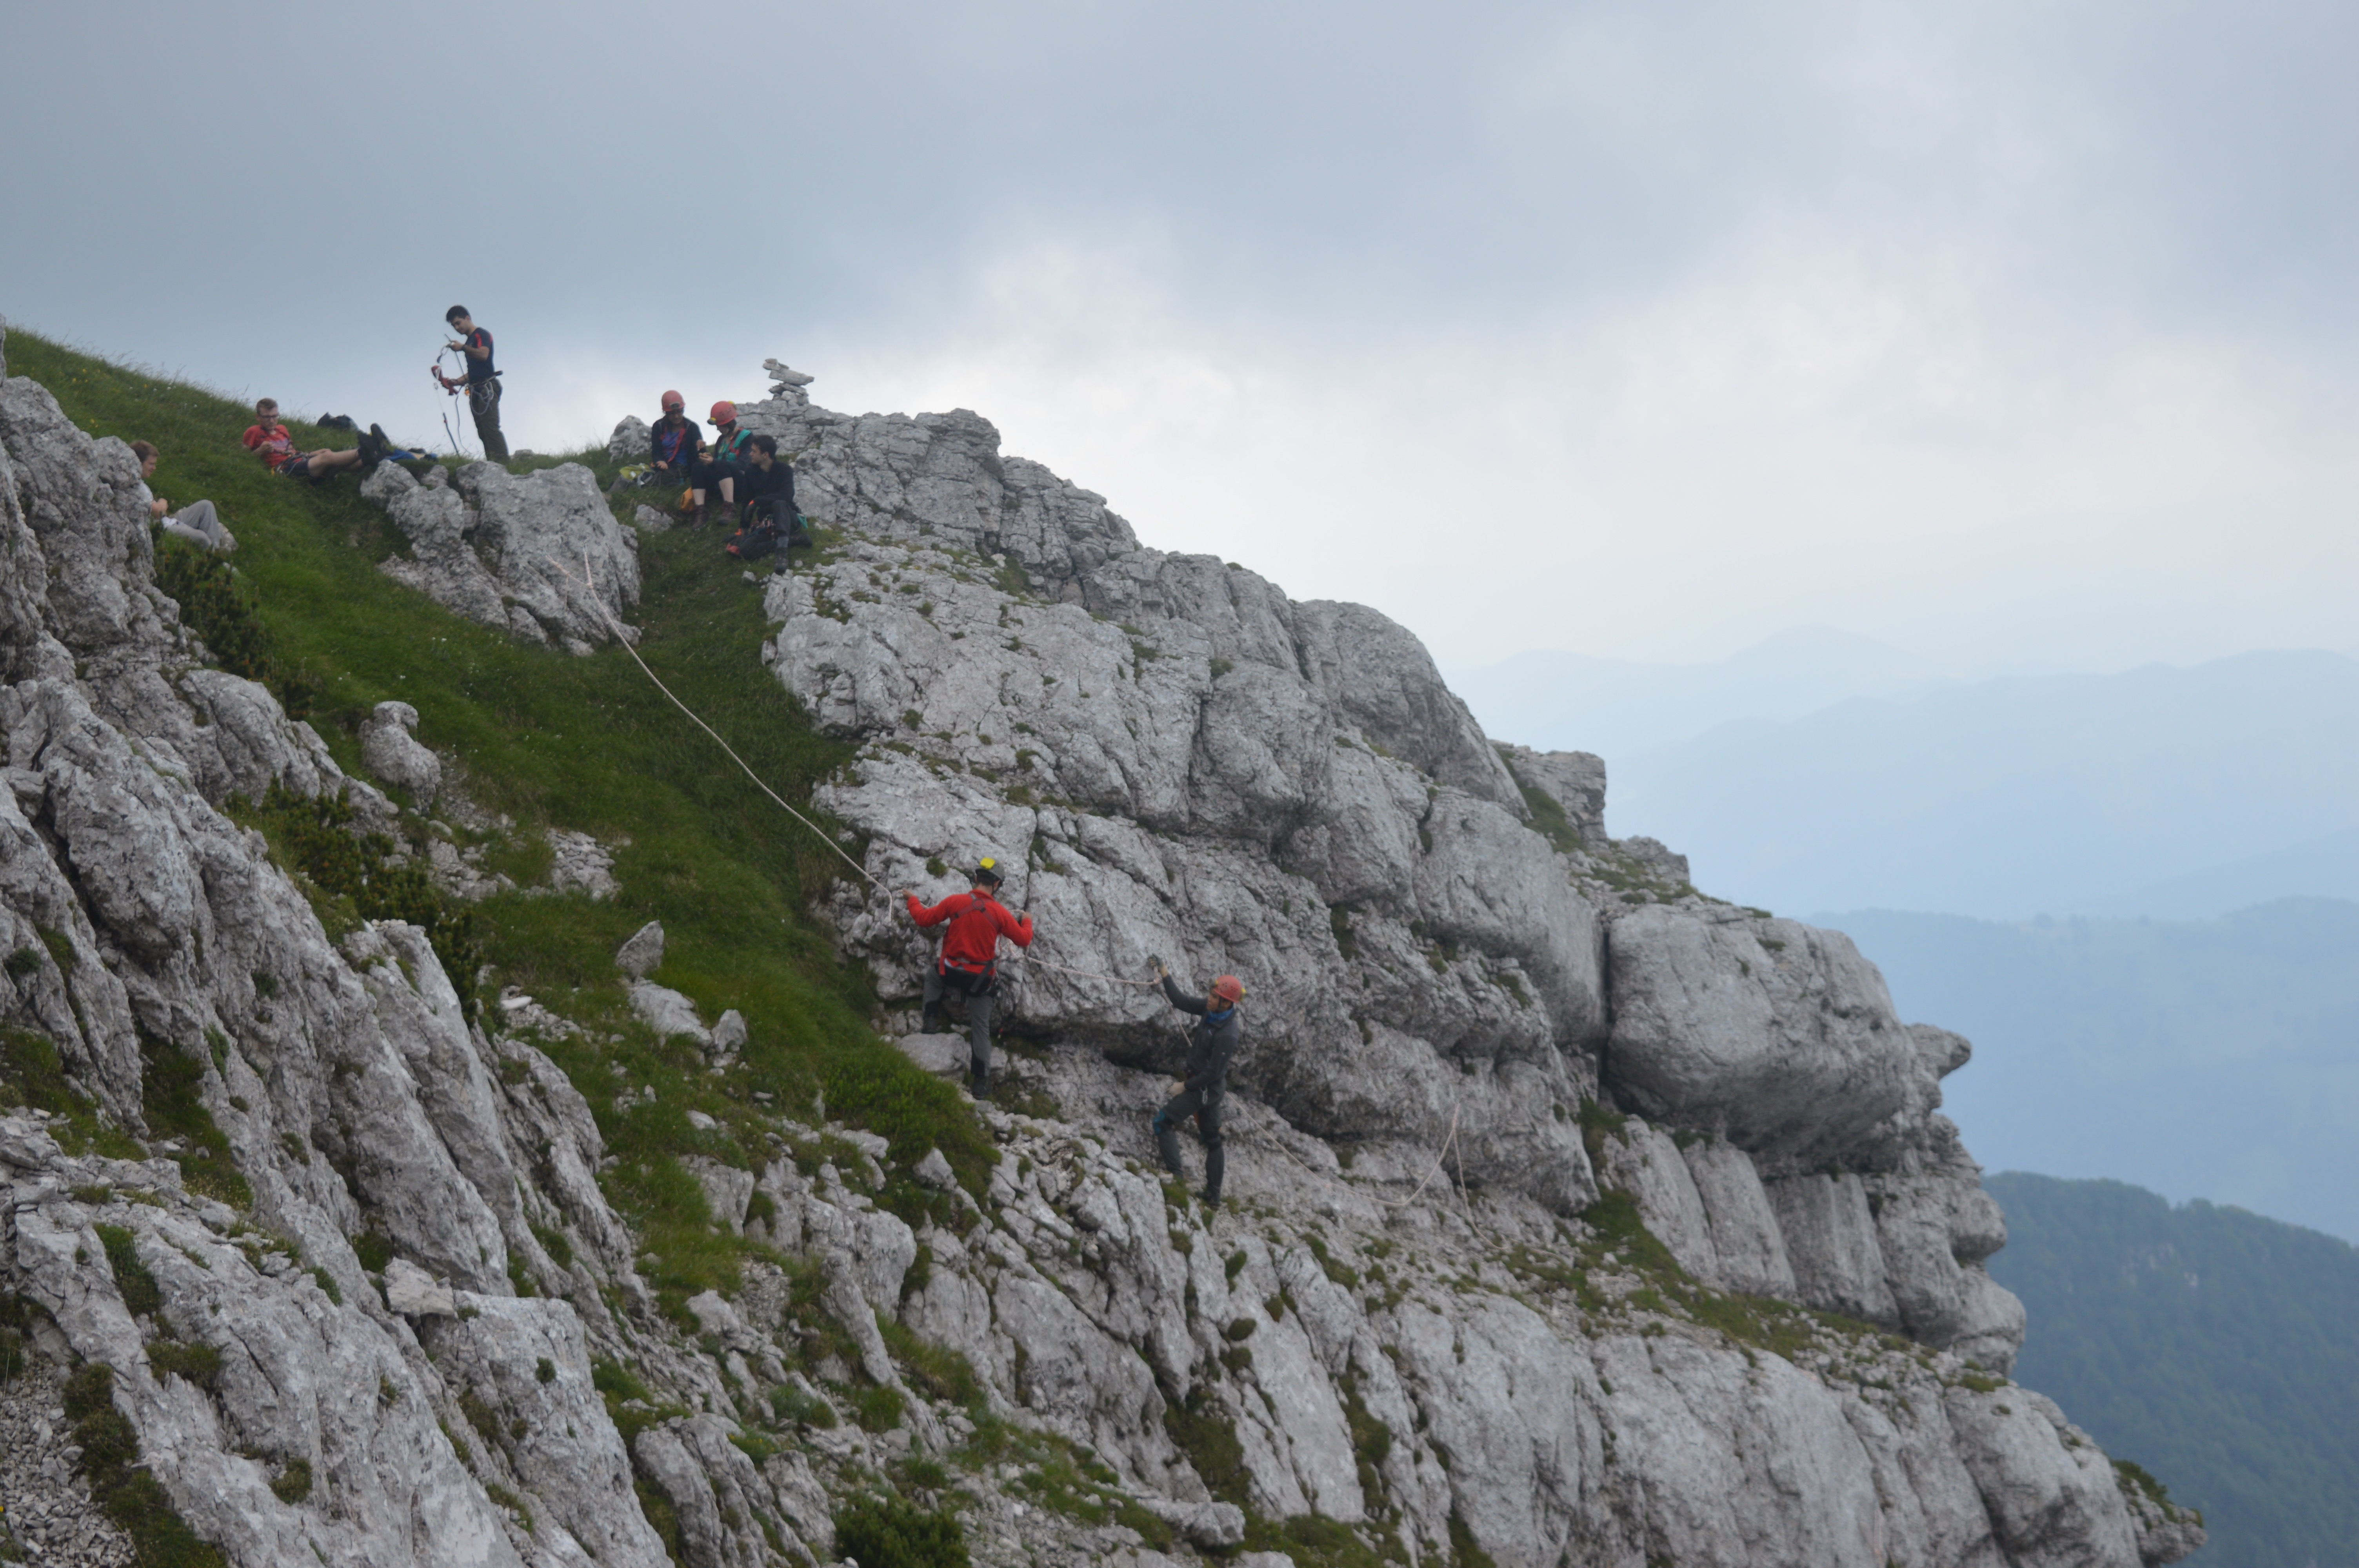
\includegraphics[width=\textwidth]{The cliff abseil.jpg}
\caption{The SRT wall above Hawk Cave --- Tanguy Racine}
\label{SRTwall}
\end{figure}

\end{document}